\documentclass[12pt, a4paper, oneside]{CIITThesissV1}
\usepackage{helvet} % Use Helvetica font as the sans-serif font
\renewcommand{\familydefault}{\sfdefault} % Set the default font family to sans-serif

\usepackage{mdframed} 
\usepackage{algorithm}
\usepackage{algorithmic}
\usepackage{placeins}
\usepackage{multirow}
\usepackage{sectsty}
\usepackage{graphicx}
\usepackage{graphics}
\usepackage[table]{xcolor}
\usepackage{lscape}
\usepackage[autostyle]{csquotes}
\usepackage{amsfonts}
\usepackage{amstext}
\usepackage{amssymb}
\usepackage[english]{babel}
\usepackage{parskip}
\usepackage[export]{adjustbox}
\usepackage{pbox}

\usepackage{afterpage}  % For better page handling

\usepackage{threeparttable}  
\usepackage{booktabs}
\usepackage{multirow}
\usepackage{bm}


\usepackage{hhline}%%%
\usepackage{pdfpages}
\usepackage{rotating}
\usepackage{epsfig}
\usepackage{booktabs}
\usepackage{float}
\usepackage{url}
\usepackage{nomencl}
\usepackage{amsmath}
\usepackage[utf8]{inputenc}
\usepackage{xcolor}
\usepackage{color, colortbl}
\usepackage{lipsum}
\usepackage{setspace}
\usepackage{afterpage}
\usepackage{pdflscape}
\usepackage{pstricks}
%\usepackage{subfigure}
\usepackage{titlesec}
\usepackage{cases}
\usepackage{tocloft}
\usepackage[numbers]{natbib}
\usepackage{amsmath}
\usepackage[hypcap=false]{caption}
\usepackage{authblk}
\usepackage{rotating}
\usepackage{pifont}
\usepackage{url}
\usepackage{array}
% \usepackage{enumitem}
\usepackage{bookmark}
\usepackage{arydshln}
\usepackage{booktabs}
\usepackage{amsmath,amssymb,amsfonts}
%\usepackage[ruled,linesnumbered]{algorithm2e}
%The following line is added to support the algorithms.
% \usepackage[ruled,vlined]{algorithm2e}
\usepackage{graphicx}
\usepackage{subcaption}
\usepackage{hyperref}
%\usepackage{longtable}
\usepackage[toc,page]{appendix}
\usepackage{matlab}
\usepackage{listings}
\lstset{breaklines=true}
\usepackage{lineno}
\usepackage{mfirstuc}
% \usepackage{pdflscape}
% \usepackage{geometry}

\usepackage{fancyhdr}

\usepackage{xltabular} % Extended tabular with auto page break and X columns
\usepackage{booktabs} % For better table formatting
\usepackage[table]{xcolor} % For cell coloring
\usepackage{makecell} % For line breaks within cells
\usepackage{listings} % For including code-like listings
\usepackage{xcolor} % For color definitions in listings
\usepackage{paralist}
%\usepackage{enumitem} % For better control over list
\usepackage[T1]{fontenc}
\usepackage{lmodern} % Latin Modern font which supports a wider range of sizes

\usepackage{microtype} % Improves typography
\usepackage{tikz}

\usepackage[most]{tcolorbox}
\usepackage{titlesec}
\usepackage{pdflscape}
\usepackage{hyperref}
\usepackage[table,xcdraw]{xcolor}
\usepackage{pgfgantt}
\usepackage{tikz}
\usepackage{titlesec}
\usepackage{amssymb}

\usepackage{colortbl}
\newcommand{\tickYes}{\checkmark}
\newcommand{\tickNo}{\texttimes}
\usetikzlibrary{fit}


\makeatletter
\def\BState{\State\hskip-\ALG@thistlm}
\graphicspath{{figures/}}
\makeatother

\renewcommand\cftchapfont{\textbf\normalfont}
\renewcommand\cftchappagefont{{\normalfont}}
\AtBeginDocument{\renewcommand\contentsname{TABLE OF CONTENTS}}
%\AtBeginDocument{\renewcommand\contentsname{\leftline{LIST OF FIGURES}}}
\titleformat{\chapter}[display]
{\bfseries\Large}
{\vspace{4cm}\centering\bigskip \Large\bfseries{Chapter \thechapter}}
{1ex}
{\bfseries\Large\centering}

% Use of colour
\usepackage{xcolor}

% Use of URL
\usepackage{url}

\definecolor{myRoyalBlue}{HTML}{4169E1}
\definecolor{myMagenta}{HTML}{FF00FF}
\definecolor{myAquaMarine}{HTML}{7FFFD4}
\definecolor{myPurple}{HTML}{A020F0}
\definecolor{myCoral}{HTML}{FF7F50}
\definecolor{SeaGreen}{HTML}{2E8B57}

% Added by Alex: BEGIN

\usepackage{enumitem}

\newenvironment{structure}[1]
    {\color{blue}
    \noindent
    \S~#1
    \begin{itemize}[leftmargin=1em,
        itemsep=.1em,
        parsep=.1em,
        topsep=.1em,
        partopsep=.1em]}
    {\end{itemize}\vspace{0.5em}}

\usepackage{soul} % For underlining
\soulregister\cite7
\soulregister\ref7

% TODO items, notes, and comments
%
% NOTE Alexandros Koliousis
\newcommand{\alex}[1]{{\color{myRoyalBlue}[\textsc{Alex:} {#1}]}}

% COMMENT Alexandros Koliousis
\newcommand{\alexcomment}[2]{\ul{#1}~{\color{myRoyalBlue}[\textsc{Alex:}] {#2}}}

\usepackage{xspace}

\newcommand{\gap}{\textcolor{red}{\textbf{[...]}}\xspace}

% END

\begin{document}
\pagenumbering{roman}

\makeatletter
\if@twocolumn
  \setlength{\marginparwidth}{20mm}
  \newcommand{\nb}[1]
  {%
   \begingroup%
   \ifodd\value{page}
     \if@firstcolumn\reversemarginpar\fi
   \else
     \if@firstcolumn\else\reversemarginpar\fi
   \fi
   \textcolor{red}{\bf!!}%{\color{red}\it\par[[#1]]\par}
   \marginnote[%\parbox{\marginparwidth}
{\scriptsize\textcolor{red}{#1}}]%
   {%\parbox{\marginparwidth}
{\scriptsize\textcolor{red}{#1}}}%
   \endgroup%
  }
\else
  \setlength{\marginparwidth}{40mm}
  \newcommand{\nb}[1]{\textcolor{red}{\bf!}%
    \reversemarginpar
    \marginpar[\parbox{\marginparwidth}{\scriptsize\textcolor{red}{\raggedleft #1}}]%
    {\parbox{\marginparwidth}{\scriptsize\textcolor{red}{\raggedright #1}}}}
\fi
\makeatother


\newtheorem{example}{Example}



\renewcommand{\S}{\mathcal{S}}
\newcommand{\D}{\mathcal{D}}
\newcommand{\F}{\mathcal{F}}
\newcommand{\T}{\mathcal{T}}

\newcommand{\adv}{\textsc{adv}}
\newcommand{\noise}{\textsc{noi}}
\newcommand{\translation}{\textsc{tra}}
\newcommand{\scale}{\textsc{sca}}
\newcommand{\shear}{\textsc{she}}
\newcommand{\rotation}{\textsc{rot}}
\newcommand{\contrast}{\textsc{con}}
\newcommand{\brightness}{\textsc{bri}}
\newcommand{\blur}{\textsc{blu}}
\newcommand{\occlusion}{\textsc{occ}}


\newcommand{\gaussian}{\textsc{gau}\xspace}
\newcommand{\saltpepper}{\textsc{sap}}

\newcommand{\testifai}{\textsc{TestifAI}\xspace}
\newcommand{\avec}[1]{\boldsymbol{#1}}



\begin{center}

\LARGE \capitalisewords {A Novel Testing Framework for Vision Models Using Bayesian Network}

\end{center}

\begin{center}
%\begin{figure}
	\includegraphics[width=6cm]{nu_logo.jpeg}
%\end{figure}
\end{center}
\begin{center}
\emph{\large By}\\

\Large {\href{https://scholar.google.com/citations?hl=en&user=ZEwBUxwAAAAJ&view_op=list_works&authuser=1&gmla=AILGF5XqzU9IqXxSuitd8SwCxQWSLHy9OoSQ59cgiyOt3Pi35gv5n8bJg_gLqFhg9SZZv2U2fvQ7DMDOmR6oiGnT5TQkhZ-vwzUvrJNRPEY2m2XMukSMolIK07cvFv6HJGZ6fEN2UhAmB9NIRd1pNy95LBWH7vzvwukF9plB9Ag}{\color{blue} Arooj Arif}}\\
\Large aa3506phd\
\vfill
\Large Mini-thesis is submitted for the probation review of PhD\\
\Large July 2024\\
% \Large Computer Science
\end{center}
\vfill

\begin{center}
\Large Northeastern University London, London - UK
\end{center}

\begin{center}
\LARGE Spring, 2024
\end{center} 
\thispagestyle{empty}



\addcontentsline{toc}{chapter}{Abstract}
\begin{center}
%{{\fontsize{16}{15} \bf ABSTRACT}\\}
{\fontsize{16}{15} \bf ABSTRACT}
\vspace{0.4cm}
\end{center}
\normalsize

Deep neural networks (DNNs) are critical in high-stake domains such as autonomous driving, medical diagnostics, and security systems, where their deployment in real-world scenarios requires rigorous robustness testing due to diverse environmental conditions. Traditional metrics like neuron coverage, while essential, do not fully capture all corner cases, which can lead to unexpected model failures. To address this gap, this research introduces a comprehensive testing framework that enhances the correctness evaluation of models through a structured five-stage process. The first stage is specification, defines essential system properties to guide the entire testing process and ensure comprehensive coverage. The second sampling stage, gathering relevant samples for exhaustive model testing. In the test case generation stage, the defined properties are applied to create targeted test scenarios. The testing and probabilistic graph stage validates the effectiveness of these test cases and conducts robustness assessments both locally (within individual category) and globally (across multiple scenarios), employing a Problog for detailed probabilistic and quantitative analysis of performance. The final stage is error summarisation, compiles and analyzes recorded errors to generate actionable graphical error reports and recommendations, thus guiding the refinement of models. This framework not only fills existing gaps in DNNs testing but also supports the development of models that are correct across varied environmental conditions.

\clearpage



  % -*- Mode:TeX -*-
%% This file simply contains the commands that actually generate the table of
%% contents and lists of figures and tables.  You can omit any or all of
%% these files by simply taking out the appropriate command.  For more
%% information on these files, see appendix C.3.3 of the LaTeX manual.
\setcounter{secnumdepth}{5}
\tableofcontents
\let\cleardoublepage\clearpage
\newpage
%\listoffigures
%let\cleardoublepage\clearpage
%\newpage
%\listoftables
%\let\cleardoublepage\clearpage
%\newpage
%\listofalgorithms
%\let\cleardoublepage\clearpage


\include{figures}
\addcontentsline{toc}{chapter}{List of Tables}
\listoftables 
\clearpage
\addcontentsline{toc}{chapter}{List of Algorithms}
\listofalgorithms
\clearpage


% \addcontentsline{toc}{chapter}{List of Symbols}
\chapter*{List of Abbreviations and Symbols}
%\markright{List of Symbols}

\begin{longtable}{ l l}

% J1 Symbols

% BC & Blockchain \\
% RSU & RoadSide Unit \\
% ITS & Intelligent Transport System \\ 
% MANET & Mobile Ad-hoc Network \\
% V2V & Vehicle to Vehicle \\ 
% V2I & Vehicle to Infrastructure \\ 
% OBU & On-Board Unit \\ 
% DSRC & Dedicated Short-Range Communication \\ 
% SPoF & Single Point of Failure \\ 
% DLT & Distributed Ledger Technology \\ 
% ECC & Elliptic Curve Cryptography \\
% P2P & Peer to Peer \\ 
% CA	& Certificate Authority		\\
% ECDSA	& Elliptic Curve Digital Signature Algorithm	\\
% PoAR & Proof of Ad Receiving \\
% CF  & Cuckoo Filter \\
% IPFS & Interplanetary Filesystem \\
% SSS & Shamir Secret Sharing \\


% $V_{s}$ & Ad sender vehicle \\
% $V_{r}$ & Ad receiving vehicle \\

% $G$ & Generator of elliptic group \\
% $h$ & Number of Ad fragments \\
% $PK$ & Public Key \\
% $PR$ & Private Key (Secret Key) \\
% $Sig$ & Digital Signature \\
% $Cert$ & Pseudonym Certificate \\
% $Link$ & Linkability between RID and PID\\
% $M$ & Ad message\\
% $TI$ & deadline (Time Threshold)\\

% %J2 symbols

% $MSK$ & Master Secret Key \\ 
% $MPK$ & Master Public Key \\ 
% $RevKey$ & Revocation Key \\ 
% $RID$ & Real Identity \\ 
% $PID$ & Pseudonym Identity \\ 
% $ts$ & Timestamp \\ 
% $TxReq$ & Request Transaction \\ 
% $t$ & Threshold \\ 
% $n$ & Number of Shamir secret shares \\ 
% $V, Veh$ & Vehicle \\ 
% $req()$ & Request \\ 
% $Enc()$ & Encryption Function \\ 






	\end{longtable}

\clearpage

\pagenumbering{arabic}
%----------------------------------

\pagestyle{fancy}
\fancyhead[LO]{\slshape \leftmark}

\rfoot{\emph{Thesis by: Arooj Arif}}


\addcontentsline{toc}{chapter}{Abstract}
\begin{center}
%{{\fontsize{16}{15} \bf ABSTRACT}\\}
{\fontsize{16}{15} \bf How to read this document}
\vspace{0.4cm}
\end{center}
\normalsize

This thesis uses terms such AI system, deep learning models, system or DNNs, interchangeably in this document. Terms related to classes in dataset (supervised learning case) such as component or class, are also used interchangeably.

\textbf{Important reading notes:}

     Terms that are used but not defined/explained in the text are listed and defined in the \textbf{GLOSSARY}. They are displayed in \textsc{small caps} in the text. Clicking on a word shown in \textsc{small caps} (e.g., \textsc{Local coverage}) takes the reader directly to the definition of that term in the Glossary. From there, one may click on the page number shown at the end of the definition to return.



\clearpage


% Adjusting chapter title format for regular (numbered) chapters
\titleformat{\chapter}[display]
  {\normalfont\huge\bfseries\centering}{\chaptertitlename\ \thechapter}{20pt}{\Huge}

% Using similar styling for unnumbered chapters but without "Chapter" prefix
\titleformat{name=\chapter,numberless}
  {\normalfont\huge\bfseries\centering}{}{0pt}{\Huge}

\titlespacing*{\chapter}{0pt}{50pt}{40pt} % Adjust vertical spacing before and after the title

\chapter{Introduction} % Ensures chapter numbering starts correctly

\section{Context} % This will now be Section 1.1, not 0.1

Deep Neural Networks (DNNs) are increasingly being used in diverse applications due to their ability to match or exceed human-level performance. The availability of large datasets, fast computing methods, and their high performance has paved the way for DNNs in safety-critical applications such as autonomous driving, medical diagnosis, and security. The safety-critical nature of such applications makes it imperative to adequately test these DNNs before deployment. However, unlike traditional software, DNNs do not have a clear control-flow structure. They learn their decision policy through training on large datasets, adjusting parameters gradually using various methods to achieve the desired accuracy. Consequently, traditional software testing methods like functional coverage and branch coverage cannot be applied to DNNs, thus challenging their use in safety-critical applications.

Recent work, discussed in Chapter II, has focused on developing testing frameworks for DNNs. These methods suffer from certain limitations, as discussed in the challenges section. In our work, we aim to overcome these limitations and build a fast, scalable, efficient, and generalizable testing framework for deep neural networks.

In this section of the thesis, the background and motivation, research questions, contributions, and organization of the thesis are presented.

\section{Background and Motivation}

In recent years, DNNs have made remarkable progress in achieving human-level performance. With the broader deployment of DNNs in various safety-critical systems like autonomous vehicles, healthcare, and avionics, concerns over their safety and trustworthiness have been raised, particularly highlighted by incidents involving self-driving cars.

An important requirement for DNNs is robustness against input perturbations. DNNs have been shown to lack robustness due to their susceptibility to adversarial examples, where small modifications to an input, sometimes imperceptible to humans, can make the network unstable.

This thesis examines existing testing methods for DNNs, opportunities for improvement, and the need for a fast, scalable, generalizable end-to-end testing method.

Coverage criteria for traditional software programs, such as code coverage and branch coverage, ensure that all parts of the logic in the program have been tested by at least one test input and all conditions have been tested to independently affect the entailing decisions. Similarly, any coverage criterion for DNNs must ensure that all parts of the internal decision-making structure of the DNN have been exercised by at least one test input.

Generating or selecting test inputs in a guided manner usually has two major goals: maximizing the number of uncovered faults and maximizing the coverage.

Testing DNNs for correctness involves verifying behaviors against a ground truth or oracle. The traditional approach of collecting and manually labeling real-world data is labor-intensive. Another method compares outputs across multiple DNNs for the same task, identifying discrepancies as corner cases. However, this can misclassify inputs if all models agree, due to shared biases or errors. This comparative approach is further limited to tasks with multiple reliable models, which may not always be available, especially in innovative or specialized applications.


\subsection{Challenges of Deep Learning Models}

The growing use of DNNs in safety-critical applications necessitates adequate testing to detect and correct any incorrect behavior for corner case inputs before deployment. DNNs lack an explicit control-flow structure, making it impossible to apply traditional software testing criteria such as code coverage.

\begin{itemize}
	\item The input space is extremely large, making unguided simulations highly unlikely to find erroneous behavior.
\end{itemize}
\subsection{Challenges in Testing of Deep Learning Models}

Unlike traditional software, DNNs do not have a clear control-flow structure. They learn their decision policy through training on a large dataset, adjusting parameters gradually using several methods to achieve desired accuracy. Consequently, traditional software testing methods like functional coverage, branch coverage, etc., cannot be applied to DNNs, thereby challenging their use in safety-critical applications. Traditional software testing methods fail when applied to DNNs because the code for deep neural networks holds no information about the internal decision-making logic of a DNN.

DNN testing techniques aim to discover bugs by finding counterexamples that challenge the system's correctness or to establish confidence by rigorously evaluating the system with numerous test cases. These testing techniques are computationally less expensive and therefore can work with state-of-the-art DNNs. However, DL testing has some limitations:
\begin{itemize}
    \item Standards available in the industry but \textbf{Lack of Logical Structure} and \textbf{System Specification}
    \item Heavily dependent on manual collections of test data under different conditions, which become expensive as the number of test conditions increases
    \item Existing coverage criteria are not detailed enough to notice subtle behaviors exhibited by DL systems
\end{itemize}

\begin{figure*}[h]
	\centering
	\includegraphics[width=0.8\textwidth]{fig1.png}
	\caption{The internal logic of a deep neural network is opaque to humans, unlike the well-laid-out decision logic of traditional software programs \cite{Intro_1}}
	\label{fig:1}
\end{figure*}

\begin{figure*}[h]
	\centering
	\includegraphics[width=0.8\textwidth]{fig2.png}
	\caption{A high-level representation of most existing DNN testing methods \cite{Intro_1}}
	\label{fig:2}
\end{figure*}



\section{Thesis Statement}

Deep learning models are being more widely used in various applications, yet their reliability in practical applications remains a challenge.


The research conducted in this thesis is driven by high-level questions that address significant challenges in the field of deep neural networks (DNNs). These questions are designed to ensure that the developed solutions not only solve specific issues but also contribute to broader goals of enhancing the reliability and robustness of DNNs in safety-critical applications.

\subsection{Research Questions and Broader Goals}

\begin{enumerate}
    \item \textbf{How can we sample inputs efficiently?}
        \begin{itemize}
            \item \textbf{Broader Goal (BG1):} Improve the robustness and accuracy of DNNs by ensuring comprehensive test coverage.
            \item \textbf{Research Objective:} Develop a hybrid sampling approach combining Borderline-SMOTE and ADASYN to enhance handling of corner cases.
        \end{itemize}
    
    \item \textbf{How can we design a comprehensive framework to test system robustness?}
        \begin{itemize}
            \item \textbf{Broader Goal (BG2):} Ensure that DNNs are reliable and safe for deployment in safety-critical applications.
            \item \textbf{Research Objective:} Create a robust framework that systematically evaluates DNN performance, reliability, and robustness.
        \end{itemize}
    
    \item \textbf{How can we systematically evaluate the robustness both at local (property-specific) and global (overall system) levels within the framework?}
        \begin{itemize}
            \item \textbf{Broader Goal (BG3):} Provide a thorough assessment of DNN robustness across different levels and scenarios.
            \item \textbf{Research Objective:} Integrate advanced probabilistic methods to evaluate both local and global robustness, providing comprehensive error summaries.
        \end{itemize}
    
    \item \textbf{Can SHAP values be used for test case generation?}
        \begin{itemize}
            \item \textbf{Broader Goal (BG4):} Enhance the interpretability and reliability of DNN testing processes.
            \item \textbf{Research Objective:} Implement SHAP analysis to identify and prioritize key influential features in the DNN testing process.
        \end{itemize}
    
    \item \textbf{How can error summarization be employed to quantify the impacts on model robustness?}
        \begin{itemize}
            \item \textbf{Broader Goal (BG5):} Facilitate targeted and effective model refinement by identifying weaknesses.
            \item \textbf{Research Objective:} Innovate error summarization techniques that identify and quantify model weaknesses.
        \end{itemize}
\end{enumerate}

\section{Research Objectives}

The primary high-level objectives of this thesis are as follows:

\begin{enumerate}

  \item \textbf{Develop Efficient Input Sampling Techniques:}
    
  \begin{itemize}
      \item \textbf{Linked to Q1 and BG1:} Create a hybrid sampling approach combining Borderline-SMOTE and ADASYN to enhance handling of corner cases and ensure comprehensive test coverage.
  \end{itemize}

    \item \textbf{Develop a Comprehensive Testing Framework for Deep Neural Networks (DNNs):}
    
    \begin{itemize}
        \item \textbf{Linked to Q2 and BG2:} Create a robust framework that systematically evaluates the performance, reliability, and robustness of DNNs, particularly in safety-critical applications.
    \end{itemize}
    
    \item \textbf{Integrate Advanced Techniques for Correctness and Robustness Evaluation:}
    
    \begin{itemize}
        \item \textbf{Linked to Q3, Q5, and BG3, BG5:} Combine traditional local correctness calculations with global correctness evaluations using advanced probabilistic methods like Problog, and develop methods to assess both local (specific properties) and global (overall system) robustness, providing comprehensive error summaries to guide improvements in model design and training.
    \end{itemize}
    
    \item \textbf{Enhance Interpretability through SHAP Analysis:}
    
    \begin{itemize}
        \item \textbf{Linked to Q4 and BG4:} Implement SHAP (SHapley Additive exPlanations) analysis to identify and prioritize key influential features in the DNN testing process.
    \end{itemize}
    
\end{enumerate}


% \begin{tcolorbox}[colback=blue!5!white, colframe=blue, title=Research Questions]

%   \smallskip\noindent%
%   \textbf{Research Questions}\hypertarget{researchquestions}{}
  
%   \begin{itemize}
%       \item \textcolor{blue}{How can we sample inputs efficiently? How can a hybrid sampling approach combining Borderline-SMOTE and ADASYN improve the handling of corner cases and enhance the robustness and accuracy of deep neural networks compared to using each technique individually?}
%       \item How can we design a comprehensive framework to test system robustness?
%       \item How can we systematically evaluate the robustness both at local (property-specific) and global (overall system) levels within the framework?
%       \item \textcolor{blue}{Can SHAP values be used for test case generation?}
%       \item How can error summarization be employed to quantify the impacts on model robustness?
%   \end{itemize}
  
%   % \end{tcolorbox}
  
%   \smallskip\noindent%
%   The above research questions guide the investigation and aim to address the challenges associated with testing deep neural networks (DNNs). These questions help to frame the specific objectives that this thesis seeks to achieve. 
  
%   \section{Research Objectives}
  
%   \textcolor{blue}{The primary high-level objectives of this thesis are as follows:}
  
%   \begin{enumerate}
%     \item \textcolor{blue}{\textbf{Develop a Comprehensive Testing Framework for Deep Neural Networks (DNNs):}
%     Create a robust framework that systematically evaluates the performance, reliability, and robustness of DNNs, particularly in safety-critical applications.}
    
%     \item \textcolor{blue}{\textbf{Integrate Advanced Techniques for Correctness and Robustness Evaluation:}
%     Combine traditional local correctness calculations with global correctness evaluations using advanced probabilistic methods like Problog, and develop methods to assess both local (specific properties) and global (overall system) robustness, providing comprehensive error summaries to guide improvements in model design and training.}
    
%     \item \textcolor{blue}{\textbf{Enhance Interpretability through SHAP Analysis:}
%     Implement SHAP (SHapley Additive exPlanations) analysis to identify and prioritize key influential features in the DNN testing process.}
    
%     % \item \textcolor{blue}{\textbf{Innovate Error Summarization Techniques:}
%     % Propose and implement new techniques for error summarization that identify and quantify model weaknesses, facilitating more targeted and effective model refinement.}
% \end{enumerate}


% \section{Thesis Contributions}\hypertarget{contributions}{}

% This research makes the following key contributions to the field of deep learning robustness evaluation:
% \begin{itemize}
%     \item We design an \textbf{end-to-end pipeline} for evaluating the correctness of the system.
%     \item We propose a \textbf{conceptual framework} that quantifies both local and global correctness, with a formalized Bayesian probabilistic approach to verify system robustness.
%     \item A novel \textbf{error summarization} approach which allows better identification of model weaknesses related to class and property.
%     \item We perform all our \textbf{experiments} using publicly available deep learning models and datasets.
% \end{itemize}

\section{Organization of the Thesis}\hypertarget{organization of thesis}{}
The remainder of the thesis is organized as follows: related studies are presented in Chapter \ref{chp:2}. The system model and proposed methodology are demonstrated in Chapter \ref{chp:3}. Chapter \ref{chp:4} describes the simulation results of our proposed schemes. Finally, the findings of this work along with future directions are presented in Chapter \ref{chp:9}.




\clearpage

\titleformat{\chapter}[display]
  {\normalfont\huge\bfseries\centering}{\chaptertitlename\ \thechapter}{20pt}{\Huge}

% Using similar styling for unnumbered chapters but without "Chapter" prefix
\titleformat{name=\chapter,numberless}
  {\normalfont\huge\bfseries\centering}{}{0pt}{\Huge}

\titlespacing*{\chapter}{0pt}{50pt}{40pt} % Adjust vertical spacing before and after the title


\chapter{Literature Review} % Ensures chapter numbering starts correctly
\label{chp:2}
\section{Overview} % This will now be Section 1.1, not 0.1

\subsection{Coverage Criteria for Deep Learning Models}

\begin{table}[h]
    \centering
    \begin{tabular}{|p{4cm}|p{5cm}|p{5cm}|}
    \hline
    \textbf{Existing Coverage Methods} & \textbf{Description} & \textbf{Limitation} \\
    \hline
    Neuron Coverage & Measures the model's logic use by counting activated neurons from test inputs. & Doesn't capture all potential DNN behaviors and can achieve high coverage with few inputs; it is a coarse measure. \\
    \hline
    k-Multisection Neuron Coverage & Divides neuron activation values observed during training into k buckets and counts how many buckets are covered by a set of inputs. & Loses information on activations beyond the observed range during aggregation. \\
    \hline
    DeepCover & Considers condition-decision dependencies between adjacent DNN layers. & Limited to small, feedforward, fully-connected networks; doesn't generalize to complex architectures like RNNs or LSTMs. \\
    \hline
    DeepCT & Inspired by combinatorial testing, assesses logic use by the fraction of neurons activated in each layer. & Lacks consideration for inter-layer relationships and hasn't been proven to scale to real-world DNNs. \\
    \hline
    \end{tabular}
    \caption{Coverage Methods, Descriptions, and Limitations}
    \label{table:coverage_methods}
    \end{table}

\subsection{Test Case Generation for Deep Learning Models}

    


\begin{table}[h]
    \centering
    \begin{tabular}{|p{3.5cm}|p{5.5cm}|p{5.5cm}|}
    \hline
    \textbf{Existing Methods} & \textbf{Description} & \textbf{Limitation} \\
    \hline
    Joint Optimization & Modifies an existing input through image manipulations recursively until it triggers different behavior in the model. & Time-consuming and produces a low ratio of impactful test inputs compared to the total tested/generated. \\
    \hline
    Greedy Search & Applies random transformations to an existing test input until a suitable test input is identified. & Similar to joint optimization, it is also time-intensive and results in a low number of effective test inputs relative to the total tested. \\
    \hline
    \end{tabular}
    \caption{Summary of Existing Test Input Generation Methods}
    \label{table:test_input_generation_methods}
    \end{table}
    
	
\begin{table}[h]
    \centering
    \begin{tabular}{|p{6cm}|p{6cm}|}
    \hline
    \textbf{Existing Approaches} & \textbf{Limitations} \\
    \hline
    Collecting as much real-world data as possible and manually labeling it for correctness. & The process requires a lot of manual effort. \\
    \hline
    Comparing outputs across multiple DNNs for the same task, identifying discrepancies as corner cases. & Can misclassify inputs if all models agree, due to shared biases or errors. Limited to tasks with multiple reliable models, which may not always be available. \\
    \hline
    \end{tabular}
    \caption{Limitations of Existing Approaches in DNN Testing}
    \label{table:existing_approaches_limitations}
    \end{table}

\begin{landscape}
    \begin{xltabular}{\linewidth}{|>{\raggedright\arraybackslash}X|>{\raggedright\arraybackslash}X|>{\raggedright\arraybackslash}p{3.5cm}|>{\raggedright\arraybackslash}p{6cm}|>{\raggedright\arraybackslash}p{2.5cm}|>{\raggedright\arraybackslash}p{3cm}|} % Adjust '3cm' as needed
    \caption{Summary of Test Methodologies and Their Characteristics} \\
    \hline
    \rowcolor[HTML]{EFEFEF} 
    \textbf{Methodology} & \textbf{Dataset} & \textbf{Benchmark} & \textbf{Limitation/Future Work} & \textbf{Coverage Criteria} & \textbf{Test Generation} \\ \endhead
    
    Symbolic execution with local explainability. LIME provides explanations for predictions\cite{Agarwal} & German Credit Data, Adult census income, Bank marketing, US Executions, Fraud Detection, Raw Car Rentals, Credit data, Census data & THEMIS (Algorithm) The technique produces 3.72 times more successful test cases than existing state-of-the-art. & FW: Expand to text and image domains FW: Measure symbolic execution efficacy using neuron coverage, boundary value coverage. & -- & Concolic \\ \hline
    
    
    Concolic testing method \cite{Youcheng} & \makecell[lt]{ MNIST\\  CIFAR-10} & DeepXplore, DeepTest, DeepCover, and DeepGauge & & \makecell[lt]{NC, SSC, NBC} & Concolic \\ \hline
    \cellcolor[HTML]{FFFFFF}Whitebox framework for testing DL systems, introducing neuron coverage for test measurement \cite{Kexin}& \makecell[lt]{ MNIST\\ ImageNet\\ Driving\\ VirusTotal\\ Drebin} & \makecell[lt]{LeNet variations\\ State-of-the-art\\ image classifiers \\ Nvidia DAVE \\ PDF malware detectors\\ Android app\\ malware detectors} & Inherits differential testing constraints. & NC & Dual-optimisation \\ \hline
    Automates testing for DNN-driven autonomous cars \cite{Yuchi}& Udacity self driving car challenge 2 & \makecell[lt]{Chauffeur-\\ Epoch\\ Rambo-S1\\ Rambo-S2\\ Rambo-S3} & \makecell[lt]{L:missing some realistic cases.\\ L: restricted only steering angle,\\ not focus on brake and accelerator\\ L: cannot simulate complex road scene}. & NC & Greedy search \\ \hline
    White box methodology, Proposed four novel test criteria tailored to DNN, structural features. able to capture and quantify causal relations existing in a DNN, Achieved balance between bug finding ability and computational cost \cite{Sun}  & MNIST, CIFAR-10, ImageNet & State-of-the-art neural networks of different sizes (from a few hundred up to millions of neurons) to demonstrate their utility with respect to four aspects: bug finding, DNN safety statistics, testing efficiency, DNN internal structure analysis & & MC/DC & Symbolic execution \\ \hline
    Proposed criteria facilitate the understanding of DNNs as well as the test data quality from different levels and angles\cite{Ma} & \makecell[lt]{MNIST, ImageNet} & \makecell[lt]{LeNet-1\\ LeNet-4\\ LeNet-5,\\ VGG-19,\\ ResNet-50} & \makecell[lt]{More diverse datasets \\and DL architectures needed.\\ Check on real-world systems.} & NBC & Gradient descent methods \\ \hline
    An unsupervised learning framework to synthesize realistic driving scenes to test inconsistent behaviors\cite{Zhang} & Udacity Training Udacity Test Ep1 Udacity Test Ep2 Youtube Ep1 Youtube Ep2 & Autumn, Chauffeur & \makecell[lt]{Lack a good standard to evaluate image\\ quality (i.e., realism). Udacity dataset is \\relatively small and the \\autonomous driving models are \\quite simple. Only focus on steering\\ wheel.} & -- & Mutation testing \\ \hline
    An automated fuzz testing framework for hunting potential defects of general-purpose DNNs\cite{Xie} & MNIST, CIFAR-10, ImageNet & \makecell[lt]{LeNet-1\\ LeNet-4\\ LeNet-5\\ RN-20\\ VGG-16\\ MobileNet\\ RN-50} & NC cannot generate effective results to evaluate the models with various quality. NC is less effective in error triggering test detection and sensitive defect detection. & \makecell[lt]{NC\\ KMNC\\ NBC\\ SNAC\\ KNC\\ KNC} & Metamorphic mutation \\ \hline
    
    \end{xltabular}
    
    \end{landscape}
% Adjusting chapter title format for regular (numbered) chapters
\titleformat{\chapter}[display]
  {\normalfont\huge\bfseries\centering}{\chaptertitlename\ \thechapter}{20pt}{\Huge}

% Using similar styling for unnumbered chapters but without "Chapter" prefix
\titleformat{name=\chapter,numberless}
  {\normalfont\huge\bfseries\centering}{}{0pt}{\Huge}

\titlespacing*{\chapter}{0pt}{50pt}{40pt} % Adjust vertical spacing before and after the title

\chapter{Proposed Framework} % Ensures chapter numbering starts correctly
\label{chp:3}


This chapter presents a comprehensive approach for AI systems, which may consist of one or multiple DNN components, each component handle different task. My research introduces a framework that addresses each DNN separately, recognising that each has unique specifications, e.g., consider an AI system using the MNIST dataset for different purposes. One DNN might classify handwritten digits (0-9), while another might analyse pairs of digits to predict their sum or product. Although both DNNs work with digit images in this case, their properties in specifications differ due to their distinct tasks, even when using the same dataset. In other cases, such as an autonomous car, different DNNs might use different datasets designed for their specific tasks. One DNN might use labeled images for object detection (e.g., identifying pedestrians, vehicles, and road signs), while another DNN might use data on driving paths and movement for path planning to predict optimal routes. This framework provides end-to-end testing for each DNN. It consists of five components, summarized in Figure~\ref{fig:framework}.

\begin{enumerate}
  \item \emph{Specification} defines key properties to guide testing. It includes details about the DNN architecture, environmental properties, and input data, like data type, sample size, and number of classes. 
    \item \emph{Sampling} involves selecting a representative subset of inputs from a potentially vast input space. Depending on the testing objectives, this subset helps ensure that the tests are meaningful and cover various scenarios effectively.
    \item \emph{Testcase Generation} applies the properties mentioned in the specifications to the sampled data to generate test cases.
    \item \emph{Testing Graph Analysis} conducts both local and global coverage assessments. Locally, it focuses on an individual property to check its correctness. Globally, it examines multiple properties to understand their interdependencies and overall system behavior. By modeling these dependencies probabilistically, testing graph analysis provides a comprehensive view of AI system.
    \item \emph{Error Summarisation} quantify the performance of the AI system by compiling and analyzing recorded errors. This analysis generates graphical reports and recommendations, helping to refine and improve the models.
\end{enumerate}

\begin{figure*}
  \centering
  \includegraphics[width=\linewidth]{figures/fivesteps.png}
  \caption{Overview of the Proposed Framework}
  \label{fig:framework}
\end{figure*}

My research focus on AI systems with DNN components performing various tasks, which may include classification, regression, clustering and more. Each DNN within the system has unique specifications. Formally, we define an AI system $ \mathcal{S} $ as follows:

$\mathcal{F}$ is the functional unit comprises $n$ DNN components $ f_1, \dots, f_n $, each handling different tasks, and a symbolic (software) component $ \omega $ that integrates the outputs of these DNNs. Given an input $\vec{x} = (x_1, \dots, x_n)$, where each $x_i$ represents an input from the respective dataset of $f_i$, the output $\mathcal{F}(\vec{x})$ is defined as $\omega(f_1(x_1), \dots, f_n(x_n))$. Each DNN component $f_i$ processes its input $x_i$ according to its specific dataset.


\section{Specification}
The first component of this framework is formalized to specify model architecture $\mathcal{M}$, environmental properties, testing type, and input data characteristics $\mathcal{D}$. 

The specifications $\mathcal{S}_{\text{specs}}$ include all classes (classification task) by default, but users can adjust this to test specific classes based on their needs.

It is essential to specify the type of testing $\mathcal{T}$ within the $\mathcal{S}_{\text{specs}}$, as different methods are employed based on this choice. In black-box testing $\mathcal{T}_{\text{black}}$, semantic adversarial properties $\mathcal{P}_{\text{sem}}$ are applied by adjusting the input data $\mathcal{D}$ without any knowledge of the model's internal details. In white-box testing $\mathcal{T}_{\text{white}}$, adversarial attacks $\mathcal{P}_{\text{adv}}$ are used by accessing the model's internal structure and parameters. Grey-box testing $\mathcal{T}_{\text{grey}}$ combines aspects of both, utilizing partial knowledge of the model’s structure to inform the testing process. 



\begin{example}
  \label{ex:mnist-adder-specification}
  Consider the AI system $\mathcal{S}_{\text{adder}}$, an \emph{MNIST Digit Adder}, which is specified as $\mathcal{S}_{\text{adder}} = (\mathcal{F}, \mathcal{D})$. In this system, the functional unit $\mathcal{F}$ consists of a DNN component $\mathcal{M}_{\text{CNN}}$, which is a Convolutional Neural Network (CNN) designed to recognize digits ranging from 0 to 9. The dataset $\mathcal{D}$ provides input in the form of images, and a software component $\omega$ is used to perform the addition of the recognized digits. 

  Formally, we define $\mathcal{F} = (\{\mathcal{M}_{\text{CNN}}\}, \omega)$, where $\omega$ integrates the output of the DNN. The function $\mathcal{M}_{\text{CNN}}$ takes single digit as an input and recognizes the digits. The software component $\omega$ can then pick any two recognized digits and compute their sum. For example, $\mathcal{S}_{\text{adder}}$ can perform the task of digit addition:
  \begin{equation}
    \mathcal{S}_{\text{adder}}(x_1, x_2) = \omega(\mathcal{M}_{\text{CNN}}(x_1), \mathcal{M}_{\text{CNN}}(x_2)),
  \end{equation}
  where $\omega(a, b) = a + b$. Given two digits $x_1$ and $x_2$, $\mathcal{S}_{\text{adder}}$ recognizes the digits and computes their sum.

  The specifications $\mathcal{S}_{\text{specs}}$ for this system include the following key elements: The DNN component $\mathcal{M}_{\text{CNN}}$ is a pre-trained CNN with a typical architecture involving a convolutional layer (32 filters, kernel size 3x3, ReLU activation), followed by a max pooling layer (2x2), a flattened layer, a fully connected layer with 128 neurons (ReLU), and an output layer with 10 neurons using softmax activation. The input data $\mathcal{D}$ consists of 10,000 test samples of digits, each labeled with one of 10 classes representing the digits 0 to 9. 

  $\mathcal{S}_{\text{adder}}$ is evaluated using both black-box and white-box testing methods. In black-box testing $\mathcal{T}_{\text{black}}$, semantic adversarial properties such as rotation, brightness adjustment, blur, shear, and contrast modification are applied to the input data without accessing the internal structure of $\mathcal{M}_{\text{CNN}}$. Specifically, $\mathcal{S}_{\text{adder}}$ robustness is tested against rotations within a range of 3 to 30 degrees and brightness adjustments between 0.5 and 1.5. In white-box testing $\mathcal{T}_{\text{white}}$, adversarial examples are generated by utilizing the internal structure and parameters of $\mathcal{M}_{\text{CNN}}$, like Fast Gradient Sign Method (FGSM), Projected Gradient Descent (PGD), AdamPGD, and Deepfool.
\end{example}


\textbf{Note:} Grey-box testing, involving partial model access, will be explored in future work.
\section{Sampling}
The sampling process is designed to identify both efficient and corner cases, focusing on hard-to-learn examples to enhance the robustness of the model. Data is sampled according to the requirements specified in the specifications. By default, all classes are tested, but users can customize the classes to be sampled based on specific requirements. The sampling approach is applied as follows for each classifier $f_i$ independently:

The full sample $\mathcal{X}_i$ for classifier $f_i$, $i=1,\dots,n$, is computed by applying the sampling method directly to the dataset $\mathcal{D}_i$:

\begin{equation}
\mathcal{X}_i = \text{Sampling}(\mathcal{D}_i)
\end{equation}

Here, $\mathcal{D}_i$ represents the dataset associated with each classifier $f_i$. In cases where all classifiers share the same dataset, $\mathcal{D}_i$ may be identical across all $i$, denoted simply as $\mathcal{D}$. However, if the datasets differ for each classifier, they are represented individually as $\mathcal{D}_1, \mathcal{D}_2, \dots, \mathcal{D}_n$ to reflect the specific dataset for each $f_i$.



This sampling method is designed to balance the dataset and ensure that both typical and challenging cases are adequately represented, thereby improving the evaluation of the model's performance across a variety of scenarios.


\begin{example}
  \label{ex:sampling}
  To further illustrate the sampling process, consider the classifier $\mathcal{M}_{\text{CNN}}$ and $\mathcal{D}$ from Example~\ref{ex:mnist-adder-specification}. For each class $c$ in $\mathcal{D}$, we begin with the samples specified in specification, forming the initial subset $\mathcal{X}_{\text{mnist}}$. This subset is then enhanced by applying a hybrid sampling method, that combines Borderline-SMOTE focuses on creating samples near decision boundaries, while ADASYN targets hard-to-learn examples, ensuring that both typical and challenging cases are effectively covered. The final sample $\mathcal{S}_{\text{mnist}}$ for testing is obtained as:
  

  \begin{equation}
    \mathcal{X}_{\text{mnist}} = \text{HybridSampling}(\mathcal{X}_{\text{mnist}})
  \end{equation}

  where the HybridSampling method combines Borderline-SMOTE and ADASYN. This process ensures a balanced and comprehensive set of test samples, covering both typical and challenging cases for robust evaluation of $\mathcal{M}_{\text{CNN}}$.
\end{example}




\begin{tcolorbox}[colback=purple!2!white, colframe=purple, title=Challenges in Sampling]
  \begin{itemize}
    \item \textbf{Synthetic Sample Quality:} Ensuring generated samples represent true corner cases, not noise.
    \item \textbf{Computational Overhead:} Managing the intensive computation required for hybrid sampling.
 
  \end{itemize}

\end{tcolorbox}


\section{Test Case Generation}

The test case generation process aims to create test cases based on the given specifications to evaluate the correctness/robustness of the AI system.

Let $S_i^c$ be the set of samples produced in the sampling step for the classifier $f_i$ and a class $c$. For each perturbation $p\in P$, we generate a set $\T_p^c$ of test cases. Specifically, for each sample $x\in S$ we produce $testcases(p,c,x)$ according to $p$. Then $\T_p^c = \bigcup_{x\in S} testcases(p,c,x)$.

\begin{example}
To generate test cases for the MNIST Digit Adder $\S_{\text{MNIST}}$, we use the specifications defined in Example 2, which include noise and rotation perturbations. Let $S$ be the set of sampled images obtained in Example 3. For each pair of images $(x_1, x_2) \in S$, we define the following test cases:
\begin{itemize}
    \item \textbf{Rotation}: For a given angle $\theta$, generate the perturbed images $x_1' = \text{rotate}(x_1, \theta)$ and $x_2' = \text{rotate}(x_2, \theta)$. The test case is then:
    $\mathcal{T}_{\text{rotation}} = \left\{(x_1', x_2') \mid x_1', x_2' \in \text{rotate}(S, \theta)\right\}$
    \item \textbf{Noise}: For a given mean $\mu$ and standard deviation $\sigma$, generate the perturbed images $x_1'' = \text{noise}(x_1, \mu, \sigma)$ and $x_2'' = \text{noise}(x_2, \mu, \sigma)$. The test case is then:
    $\mathcal{T}_{\text{noise}} = \left\{(x_1'', x_2'') \mid x_1'', x_2'' \in \text{noise}(S, \mu, \sigma)\right\}$
\end{itemize}
The overall set of test cases $\mathcal{T}$ is the union of the individual test cases:
$\mathcal{T} = \mathcal{T}_{\text{rotation}} \cup \mathcal{T}_{\text{noise}}$
\end{example}

\section{Validation}

The validation process aims to evaluate the correctness and robustness of the AI system under various perturbations.

Fix a perturbation \( p \in P \) and a class \( c \). For every test case in \( \mathcal{T}_p^c \), we store the results in the form:
\[ \text{Raw}_{p, c} = \Big\{\big(\text{query}(f_i, x, c), f_i(x)_c\big) \mid x \in \mathcal{T}_p^c \Big\} \]

After generating test cases, measure the AI subsystem's confidence for each class under each type of property.

\subsection{Local Robustness}

Local robustness involves evaluating the AI subsystem's performance on individual images subjected to various transformations. For each image \( x \) from a set of samples \( S_i^c \), the AI subsystem produces a confidence score \( f_i(x) \) representing its certainty in recognizing the class \( c \). The local robustness for a transformation \( T \) applied to an image \( x \) is defined as:

\[ \text{Local Robustness}(x, T) = f_i(T(x)) \]

where \( T \) can be any transformation such as noise addition, rotation, brightness adjustment, occlusion, or scaling. Each transformation is evaluated to determine its impact on the confidence score.

To quantify local robustness, we compute the accuracy for each transformation applied to the images of a specific class:

\[
\text{Local Robustness}(c, T) = \frac{1}{|S_i^c|} \sum_{x \in S_i^c} \mathbb{I}[f_i(T(x)) = c]
\]

where:
- \(\text{Local Robustness}(c, T)\) is the accuracy of the classifier \( f_i \) for class \( c \) under transformation \( T \).
- \( \mathbb{I}[f_i(T(x)) = c] \) is an indicator function that is 1 if the classifier correctly predicts the class \( c \) for the transformed image \( T(x) \), and 0 otherwise.
- \(|S_i^c|\) is the number of correctly classified images in class \( c \).

\begin{example}
Consider the class \( c = 3 \) and the transformation \( T \) being a rotation by 25 degrees. If we have three images \( x_1, x_2, x_3 \) from class \( c \), and the model correctly classifies \( x_1 \) and \( x_2 \) but misclassifies \( x_3 \), the local robustness is computed as follows:

\[
\text{Local Robustness}(3, \text{rotation}) = \frac{1}{3} (\mathbb{I}[f_i(\text{rotate}(x_1, 25)) = 3] + 
\]
\[
\mathbb{I}[f_i(\text{rotate}(x_2, 25)) = 3] + \mathbb{I}[f_i(\text{rotate}(x_3, 25)) = 3])
\]


If the indicator values are 1, 1, and 0 respectively, the local robustness would be:

\[
\text{Local Robustness}(3, \text{rotation}) = \frac{1}{3} (1 + 1 + 0) = \frac{2}{3} \approx 0.67
\]
\end{example}

\subsection{Global Robustness}

Global robustness evaluates the AI subsystem's performance across multiple images and transformations. It is an aggregate measure of how well the AI system performs under various properties on a set of images $S_i^c$.

For a given transformation $T$ and a set of images $S_i^c$, the global robustness is defined as:

$$ \text{Global Robustness}(S_i^c, T) = \frac{1}{|S_i^c|} \sum_{x \in S_i^c} \mathbb{I}[f_i(T(x)) = c] $$

This measures the average confidence score for the AI subsystem over the entire dataset when subjected to a particular transformation.

To quantify global robustness, we compute the expected confidence score over all transformations and images. Depending on whether the relationship is AND or OR, the formulas vary:

\textbf{AND Relationship:}

For an AND relationship between transformations, the global robustness is calculated as:

$$ P(\text{Property 1} \cap \text{Property 2}) = P(\text{Property 1}) \times P(\text{Property 2}) $$

\textbf{OR Relationship:}

For an OR relationship between transformations, the global robustness is calculated as:

$$ P(\text{Property 1} \cup \text{Property 2}) = P(\text{Property 1}) + P(\text{Property 2}) - P(\text{Property 1} \cap \text{Property 2}) $$

\begin{example}
Consider a pair of images $(x_1, x_2)$ representing the digits '3' and '5'. Let the transformation $T$ be rotation. If the model's confidence scores for these transformations are as follows:

$$
\begin{aligned}
&f_i(\text{rotation}(x_1)) = 0.78, \\
&f_i(\text{rotation}(x_2)) = 0.85,
\end{aligned}
$$

For the AND relationship, the global correctness for the pair is computed as follows:

$$P(\text{Global Robustness}_{\text{AND}}) = 0.78 \times 0.85$$

For the OR relationship, the global correctness for the pair is computed as follows:

$$P(\text{Global Robustness}_{\text{OR}}) = 0.78 + 0.85 - (0.78 \times 0.85)$$

(Note: The complete OR relationship formula requires including all images and transformations as per the OR formula.)

\end{example}

\subsection{Use Cases and Examples}
To illustrate the application of ProbLog for global robustness in real-world scenarios, we present the following use cases:

\subsubsection{Use Case 1: Handwritten Digit Recognition}
\textbf{Scenario:} Consider an AI system designed to recognize handwritten digits, such as the MNIST dataset. The system is evaluated under various transformations, including noise addition, rotation, and brightness adjustment. The goal is to determine the global robustness of the system in recognizing digit pairs correctly under these properties.

The tables below provide the probabilities for correctly recognizing digit pairs under different conditions (AND and OR relationships) for an MNIST 2-digit addition system. Each world represents a different combination of transformations applied to the digits.

\begin{table}[h]
    \centering
    \caption{Specification Probabilities for MNIST 2-Digit Addition Under Different Transformations}
    \label{tab:mnist_prob_and_or}
    \resizebox{\textwidth}{!}{%
    \begin{tabular}{|c|c|c|c|c|c|}
    \hline
    \textbf{World} & \textbf{Conditions} & \textbf{Probability Expression (AND)} & \textbf{Probability (AND)} & \textbf{Probability Expression (OR)} & \textbf{Probability (OR)} \\
    \hline
    $w_1$ & \{noise(0), noise(1)\} & $0.85 \cdot 0.8$ & $0.68$ & $0.85 + 0.8 - (0.85 \cdot 0.8)$ & $0.97$ \\
    $w_2$ & \{noise(0), correct(1)\} & $0.85 \cdot 0.9$ & $0.765$ & $0.85 + 0.9 - (0.85 \cdot 0.9)$ & $0.985$ \\
    $w_3$ & \{correct(0), noise(1)\} & $0.9 \cdot 0.8$ & $0.72$ & $0.9 + 0.8 - (0.9 \cdot 0.8)$ & $0.98$ \\
    $w_4$ & \{rotation(0), correct(1)\} & $0.88 \cdot 0.9$ & $0.792$ & $0.88 + 0.9 - (0.88 \cdot 0.9)$ & $0.992$ \\
    $w_5$ & \{correct(0), rotation(1)\} & $0.9 \cdot 0.77$ & $0.693$ & $0.9 + 0.77 - (0.9 \cdot 0.77)$ & $0.977$ \\
    $w_6$ & \{rotation(0), rotation(1)\} & $0.88 \cdot 0.77$ & $0.6776$ & $0.88 + 0.77 - (0.88 \cdot 0.77)$ & $0.9696$ \\
    $w_7$ & \{noise(0), rotation(1)\} & $0.85 \cdot 0.77$ & $0.6545$ & $0.85 + 0.77 - (0.85 \cdot 0.77)$ & $0.9655$ \\
    $w_8$ & \{rotation(0), noise(1)\} & $0.88 \cdot 0.8$ & $0.704$ & $0.88 + 0.8 - (0.88 \cdot 0.8)$ & $0.976$ \\
    $w_9$ & \{correct(0), correct(1)\} & $0.9 \cdot 0.9$ & $0.81$ & $0.9 + 0.9 - (0.9 \cdot 0.9)$ & $0.99$ \\
    \hline
    \end{tabular}
    }
\end{table}

\textbf{Explanation:} The table shows the global correctness probabilities for pairs of digits under various transformation conditions. Each row represents a different combination of transformations applied to the two digits in the pair:
- AND Probability: The probability that both digits are correctly recognized under the specified transformations.
- OR Probability: The probability that at least one of the digits is correctly recognized under the specified transformations.

For example, in world $w_1$, both digits are subjected to noise, leading to an AND probability of $0.68$ and an OR probability of $0.97$.

\textbf{Problog Code:}
\begin{mdframed}[leftline=false, rightline=false, topline=true, bottomline=true]
\scriptsize
\begin{verbatim}
% Define probabilities for digit 0 under different transformations
0.9::noise_0. % Digit 0 correctly predicted with 90% probability under noise
0.85::brightness_0. % Digit 0 correctly predicted with 85% probability under brightness
0.88::rotation_0. % Digit 0 correctly predicted with 88% probability under rotation

% Define probabilities for digit 1 under different transformations
0.8::noise_1. % Digit 1 correctly predicted with 80% probability under noise
0.75::brightness_1. % Digit 1 correctly predicted with 75% probability under brightness
0.77::rotation_1. % Digit 1 correctly predicted with 77% probability under rotation

% Define rules for correct prediction under each transformation for digit 0
correct_noise_0 :- noise_0.
correct_brightness_0 :- brightness_0.
correct_rotation_0 :- rotation_0.

% Define rules for correct prediction under each transformation for digit 1
correct_noise_1 :- noise_1.
correct_brightness_1 :- brightness_1.
correct_rotation_1 :- rotation_1.

% Define rules for incorrect prediction under each transformation for digit 0
wrong_noise_0 :- +correct_noise_0.
wrong_brightness_0 :- +correct_brightness_0.
wrong_rotation_0 :- +correct_rotation_0.

% Define rules for incorrect prediction under each transformation for digit 1
wrong_noise_1 :- +correct_noise_1.
wrong_brightness_1 :- +correct_brightness_1.
wrong_rotation_1 :- +correct_rotation_1.

% Define rules for correct prediction of both digits under noise
pair_correct_noise_0_1 :- correct_noise_0, correct_noise_1.
% Define rules for incorrect prediction of both digits under noise
pair_wrong_noise_0_1 :- wrong_noise_0, wrong_noise_1.

% Define global correctness based on either both correct or both incorrect under noise
global_correct_noise_0_1 :- pair_correct_noise_0_1; pair_wrong_noise_0_1.

% Query the global correctness under noise
query(global_correct_noise_0_1).
\end{verbatim}
\end{mdframed}
\captionof{figure}{Problog code snippet for evaluating handwritten digit recognition under noise, brightness, and rotation transformations.}

\textbf{Explanation:} In this scenario, we are interested in the global correctness of recognizing pairs of digits (0 and 1) under different transformations. The ProbLog code models the local robustness probabilities for each transformation and combines them to evaluate the global correctness.

\subsubsection{Use Case 2: Autonomous Vehicle Perception}

\textbf{Scenario:} An AI system used in autonomous vehicles must reliably detect objects such as vehicles under various weather conditions (rain, sand, fog, and snow). The goal is to evaluate the system's robustness in identifying these objects correctly under these weather conditions.

\begin{mdframed}[leftline=false, rightline=false, topline=true, bottomline=true]
  \scriptsize
  \begin{verbatim}

% Probabilities for Vehicle Detection under Different Weather Conditions
0.75::rain_vehicle. % Vehicle correctly detected with 75% probability under rain
0.55::fog_vehicle. % Vehicle correctly detected with 55% probability under fog
0.7::snow_vehicle. % Vehicle correctly detected with 70% probability under snow

% Correct Detection Rules for Vehicle
correct_rain_vehicle :- rain_vehicle.
correct_fog_vehicle :- fog_vehicle.
correct_snow_vehicle :- snow_vehicle.

% Incorrect Detection Rules for Vehicle
wrong_rain_vehicle :- +correct_rain_vehicle.
wrong_fog_vehicle :- +correct_fog_vehicle.
wrong_snow_vehicle :- +correct_snow_vehicle.

% AND conditions for Vehicle Detection under all weather conditions
global_correct_vehicle_and :- correct_rain_vehicle, correct_fog_vehicle, correct_snow_vehicle.

% OR conditions for Vehicle Detection under any weather condition
global_correct_vehicle_or :- correct_rain_vehicle; correct_fog_vehicle; correct_snow_vehicle.

% Mixed conditions (AND & OR) for Vehicle Detection
global_correct_mixed_vehicle :- correct_rain_vehicle, (correct_fog_vehicle; correct_snow_vehicle).

% Queries for Global Correctness
query(global_correct_vehicle_and).
query(global_correct_vehicle_or).
query(global_correct_mixed_vehicle).
\end{verbatim}
\end{mdframed}
\captionof{figure}{Problog code snippet for evaluating vehicle detection under different weather conditions.}

\textbf{Explanation:} The ProbLog code assesses the global robustness of the AI system in detecting objects (vehicles) under individual and combined weather conditions. This ensures that the system can reliably perform in diverse environmental scenarios.

\begin{table}[h]
  \centering
  \caption{Specification Probabilities (AND) for Vehicle Detection Under Different Weather Conditions \\
  \( P(A \cap B \cap C) = P(A) \times P(B) \times P(C) \)}
  \label{tab:veh_prob_and}
  \resizebox{\textwidth}{!}{%
  \begin{tabular}{|c|c|c|c|}
  \hline
  \textbf{World} & \textbf{Conditions} & \textbf{Probability Expression (AND)} & \textbf{Probability (AND)} \\
  \hline
  $w_1$ & \{rain, fog\} & $0.75 \times 0.55$ & $0.4125$ \\
  $w_2$ & \{rain, snow\} & $0.75 \times 0.7$ & $0.525$ \\
  $w_3$ & \{rain, sand\} & $0.75 \times 0.6$ & $0.45$ \\
  $w_4$ & \{fog, snow\} & $0.55 \times 0.7$ & $0.385$ \\
  $w_5$ & \{fog, sand\} & $0.55 \times 0.6$ & $0.33$ \\
  $w_6$ & \{snow, sand\} & $0.7 \times 0.6$ & $0.42$ \\
  $w_7$ & \{rain, fog, snow\} & $0.75 \times 0.55 \times 0.7$ & $0.28875$ \\
  $w_8$ & \{rain, fog, sand\} & $0.75 \times 0.55 \times 0.6$ & $0.2475$ \\
  $w_9$ & \{rain, snow, sand\} & $0.75 \times 0.7 \times 0.6$ & $0.315$ \\
  $w_{10}$ & \{fog, snow, sand\} & $0.55 \times 0.7 \times 0.6$ & $0.231$ \\
  \hline
  \end{tabular}
  }
\end{table}

\textbf{Explanation:} This table shows the global correctness probabilities for detecting vehicles under different combinations of weather conditions using AND relationships. Each row represents a different combination of weather conditions applied to the detection scenario:
- AND Probability: The probability that the vehicle is correctly detected under all specified weather conditions.

For example, in world $w_1$, the vehicle detection system is subjected to rain and fog, leading to an AND probability of $0.4125$.

\begin{table}[h]
  \centering
  \caption{Specification Probabilities (OR) for Vehicle Detection Under Different Weather Conditions \\
  \( P(A \cup B \cup C) = P(A) + P(B) + P(C) - P(A \cap B) - P(A \cap C) - P(B \cap C) + P(A \cap B \cap C) \)}
  \label{tab:veh_prob_or}
  \resizebox{\textwidth}{!}{%
  \begin{tabular}{|c|c|c|c|}
  \hline
  \textbf{World} & \textbf{Conditions} & \textbf{Probability Expression (OR)} & \textbf{Probability (OR)} \\
  \hline
  $w_1$ & \{rain; fog\} & $0.75 + 0.55 - (0.75 \times 0.55)$ & $0.8875$ \\
  $w_2$ & \{rain; snow\} & $0.75 + 0.7 - (0.75 \times 0.7)$ & $0.925$ \\
  $w_3$ & \{rain; sand\} & $0.75 + 0.6 - (0.75 \times 0.6)$ & $0.9$ \\
  $w_4$ & \{fog; snow\} & $0.55 + 0.7 - (0.55 \times 0.7)$ & $0.835$ \\
  $w_5$ & \{fog; sand\} & $0.55 + 0.6 - (0.55 \times 0.6)$ & $0.82$ \\
  $w_6$ & \{snow; sand\} & $0.7 + 0.6 - (0.7 \times 0.6)$ & $0.88$ \\
  $w_7$ & \{rain; fog; snow\} & $0.75 + 0.55 + 0.7 - (0.75 \times 0.55) - (0.75 \times 0.7) - (0.55 \times 0.7) + (0.75 \times 0.55 \times 0.7)$ & $0.966625$ \\
  $w_8$ & \{rain; fog; sand\} & $0.75 + 0.55 + 0.6 - (0.75 \times 0.55) - (0.75 \times 0.6) - (0.55 \times 0.6) + (0.75 \times 0.55 \times 0.6)$ & $0.95125$ \\
  $w_9$ & \{rain; snow; sand\} & $0.75 + 0.7 + 0.6 - (0.75 \times 0.7) - (0.75 \times 0.6) - (0.7 \times 0.6) + (0.75 \times 0.7 \times 0.6)$ & $0.967$ \\
  $w_{10}$ & \{fog; snow; sand\} & $0.55 + 0.7 + 0.6 - (0.55 \times 0.7) - (0.55 \times 0.6) - (0.7 \times 0.6) + (0.55 \times 0.7 \times 0.6)$ & $0.938$ \\
  \hline
  \end{tabular}
  }
\end{table}

\textbf{Explanation:} This table shows the global correctness probabilities for detecting vehicles under different combinations of weather conditions using OR relationships. Each row represents a different combination of weather conditions applied to the detection scenario:
- OR Probability: The probability that the vehicle is correctly detected under at least one of the specified weather conditions.

For example, in world $w_1$, the vehicle detection system is subjected to rain and fog, leading to an OR probability of $0.8875$.




% \subsection{Use Cases and Examples}

% To illustrate the application of Problog for global robustness in real-world scenarios, we present the following use cases:

% \subsection{Use Case 1: Handwritten Digit Recognition}

% \textbf{Scenario:} Consider an AI system designed to recognize handwritten digits, such as the MNIST dataset. The system is evaluated under various transformations, including noise addition, rotation, and brightness adjustment. The goal is to determine the global robustness of the system in recognizing digit pairs correctly under these properties.


  
%   \begin{table}[h]
%     \centering
  
%     \caption{Specification Probabilities for MNIST 2-Digit Addition Under Different Transformations}
%     \label{tab:mnist_prob_and_or}
  
%     \resizebox{\textwidth}{!}{%
%     \begin{tabular}{|c|c|c|c|c|c|}
%     \hline
%     \textbf{World} & \textbf{Conditions} & \textbf{Probability Expression (AND)} & \textbf{Probability (AND)} & \textbf{Probability Expression (OR)} & \textbf{Probability (OR)} \\
%     \hline
%     $w_1$ & \{noise(0), noise(1)\} & $0.85 \cdot 0.8$ & $0.68$ & $0.85 + 0.8 - (0.85 \cdot 0.8)$ & $0.97$ \\
%     $w_2$ & \{noise(0), correct(1)\} & $0.85 \cdot 0.9$ & $0.765$ & $0.85 + 0.9 - (0.85 \cdot 0.9)$ & $0.985$ \\
%     $w_3$ & \{correct(0), noise(1)\} & $0.9 \cdot 0.8$ & $0.72$ & $0.9 + 0.8 - (0.9 \cdot 0.8)$ & $0.98$ \\
%     $w_4$ & \{rotation(0), correct(1)\} & $0.88 \cdot 0.9$ & $0.792$ & $0.88 + 0.9 - (0.88 \cdot 0.9)$ & $0.992$ \\
%     $w_5$ & \{correct(0), rotation(1)\} & $0.9 \cdot 0.77$ & $0.693$ & $0.9 + 0.77 - (0.9 \cdot 0.77)$ & $0.977$ \\
%     $w_6$ & \{rotation(0), rotation(1)\} & $0.88 \cdot 0.77$ & $0.6776$ & $0.88 + 0.77 - (0.88 \cdot 0.77)$ & $0.9696$ \\
%     $w_7$ & \{noise(0), rotation(1)\} & $0.85 \cdot 0.77$ & $0.6545$ & $0.85 + 0.77 - (0.85 \cdot 0.77)$ & $0.9655$ \\
%     $w_8$ & \{rotation(0), noise(1)\} & $0.88 \cdot 0.8$ & $0.704$ & $0.88 + 0.8 - (0.88 \cdot 0.8)$ & $0.976$ \\
%     $w_9$ & \{correct(0), correct(1)\} & $0.9 \cdot 0.9$ & $0.81$ & $0.9 + 0.9 - (0.9 \cdot 0.9)$ & $0.99$ \\
%     \hline
%     \end{tabular}
%     }
%     \end{table}
  



% \textbf{Problog Code:}
% \begin{mdframed}[leftline=false, rightline=false, topline=true, bottomline=true]
% \scriptsize
% \begin{verbatim}
% % Define probabilities for digit 0 under different transformations
% 0.9::noise_0. % Digit 0 correctly predicted with 90% probability under noise
% 0.85::brightness_0. % Digit 0 correctly predicted with 85% probability under brightness
% 0.88::rotation_0. % Digit 0 correctly predicted with 88% probability under rotation

% % Define probabilities for digit 1 under different transformations
% 0.8::noise_1. % Digit 1 correctly predicted with 80% probability under noise
% 0.75::brightness_1. % Digit 1 correctly predicted with 75% probability under brightness
% 0.77::rotation_1. % Digit 1 correctly predicted with 77% probability under rotation

% % Define rules for correct prediction under each transformation for digit 0
% correct_noise_0 :- noise_0.
% correct_brightness_0 :- brightness_0.
% correct_rotation_0 :- rotation_0.

% % Define rules for correct prediction under each transformation for digit 1
% correct_noise_1 :- noise_1.
% correct_brightness_1 :- brightness_1.
% correct_rotation_1 :- rotation_1.

% % Define rules for incorrect prediction under each transformation for digit 0
% wrong_noise_0 :- +correct_noise_0.
% wrong_brightness_0 :- +correct_brightness_0.
% wrong_rotation_0 :- +correct_rotation_0.

% % Define rules for incorrect prediction under each transformation for digit 1
% wrong_noise_1 :- +correct_noise_1.
% wrong_brightness_1 :- +correct_brightness_1.
% wrong_rotation_1 :- +correct_rotation_1.

% % Define rules for correct prediction of both digits under noise
% pair_correct_noise_0_1 :- correct_noise_0, correct_noise_1.
% % Define rules for incorrect prediction of both digits under noise
% pair_wrong_noise_0_1 :- wrong_noise_0, wrong_noise_1.

% % Define global correctness based on either both correct or both incorrect under noise
% global_correct_noise_0_1 :- pair_correct_noise_0_1; pair_wrong_noise_0_1.

% % Query the global correctness under noise
% query(global_correct_noise_0_1).
% \end{verbatim}
% \end{mdframed}
% \captionof{figure}{Problog code snippet for evaluating handwritten digit recognition under noise, brightness, and rotation transformations.}



% \textbf{Explanation:} In this scenario, we are interested in the global correctness of recognizing pairs of digits (0 and 1) under different transformations. The Problog code models the local robustness probabilities for each transformation and combines them to evaluate the global correctness.


%   \subsection{Use Case 2: Autonomous Vehicle Perception}

% \textbf{Scenario:} An AI system used in autonomous vehicles must reliably detect objects such as pedestrians and vehicles under various weather conditions (rain, fog, and snow). The goal is to evaluate the system's robustness in identifying these objects correctly under these weather conditions.



% \begin{mdframed}[leftline=false, rightline=false, topline=true, bottomline=true]
%   \scriptsize
%   \begin{verbatim}

%   % Probabilities for Vehicle Detection under Different Weather Conditions
%   0.75::rain_vehicle. % Vehicle correctly detected with 75% probability under rain
%   0.55::fog_vehicle. % Vehicle correctly detected with 55% probability under fog
%   0.7::snow_vehicle. % Vehicle correctly detected with 70% probability under snow

  
%   % Correct Detection Rules for Vehicle
%   correct_rain_vehicle :- rain_vehicle.
%   correct_fog_vehicle :- fog_vehicle.
%   correct_snow_vehicle :- snow_vehicle.
  
%   % Incorrect Detection Rules for Vehicle
%   wrong_rain_vehicle :- +correct_rain_vehicle.
%   wrong_fog_vehicle :- +correct_fog_vehicle.
%   wrong_snow_vehicle :- +correct_snow_vehicle.
  

%   % AND conditions for Vehicle Detection under all weather conditions
%   global_correct_vehicle_and :- correct_rain_vehicle, correct_fog_vehicle, correct_snow_vehicle.
  
%   % OR conditions for Vehicle Detection under any weather condition
%   global_correct_vehicle_or :- correct_rain_vehicle; correct_fog_vehicle; correct_snow_vehicle.
  
%   % Mixed conditions (AND & OR) for Vehicle Detection
%   global_correct_mixed_vehicle :- correct_rain_vehicle, (correct_fog_vehicle; correct_snow_vehicle).
  
%   % Queries for Global Correctness

%   query(global_correct_vehicle_and).
%   query(global_correct_vehicle_or).
%   query(global_correct_mixed_vehicle).
%   \end{verbatim}
%   \end{mdframed}
%   \captionof{figure}{Problog code snippet for evaluating  vehicle detection under different weather conditions.}
  
  

% \textbf{Explanation:} he Problog code assesses the global robustness of the AI system in detecting objects (pedestrians and vehicles) under individual and combined weather conditions. This ensures that the system can reliably perform in diverse environmental scenarios.

% \begin{table}[h]
%   \centering
%   \caption{Specification Probabilities (AND) for Vehicle Detection Under Different Weather Conditions \\
%   \( P(A \cap B \cap C) = P(A) \times P(B) \times P(C) \)}
%   \label{tab:veh_prob_and}
%   \resizebox{\textwidth}{!}{%
%   \begin{tabular}{|c|c|c|c|}
%   \hline
% \textbf{World} & \textbf{Conditions} & \textbf{Probability Expression (AND)} & \textbf{Probability (AND)} \\
%   \hline
%   $w_1$ & \{rain, fog\} & $0.75 \times 0.55$ & $0.4125$ \\
%   $w_2$ & \{rain, snow\} & $0.75 \times 0.7$ & $0.525$ \\
%   $w_3$ & \{rain, sand\} & $0.75 \times 0.6$ & $0.45$ \\
%   $w_4$ & \{fog, snow\} & $0.55 \times 0.7$ & $0.385$ \\
%   $w_5$ & \{fog, sand\} & $0.55 \times 0.6$ & $0.33$ \\
%   $w_6$ & \{snow, sand\} & $0.7 \times 0.6$ & $0.42$ \\
%   $w_7$ & \{rain, fog, snow\} & $0.75 \times 0.55 \times 0.7$ & $0.28875$ \\
%   $w_8$ & \{rain, fog, sand\} & $0.75 \times 0.55 \times 0.6$ & $0.2475$ \\
%   $w_9$ & \{rain, snow, sand\} & $0.75 \times 0.7 \times 0.6$ & $0.315$ \\
%   $w_{10}$ & \{fog, snow, sand\} & $0.55 \times 0.7 \times 0.6$ & $0.231$ \\
%   \hline
%   \end{tabular}
%   }
% \end{table}


% \begin{table}[h]
%   \centering
%   \caption{Specification Probabilities (OR) for Vehicle Detection Under Different Weather Conditions \\
%   \( P(A \cup B \cup C) = P(A) + P(B) + P(C) - P(A \cap B) - P(A \cap C) - P(B \cap C) + P(A \cap B \cap C) \)}
%   \label{tab:veh_prob_or}
%   \resizebox{\textwidth}{!}{%
%   \begin{tabular}{|c|c|c|c|}
%   \hline
% \textbf{World} & \textbf{Conditions} & \textbf{Probability Expression (OR)} & \textbf{Probability (OR)} \\
%   \hline
%   $w_1$ & \{rain; fog\} & $0.75 + 0.55 - (0.75 \times 0.55)$ & $0.8875$ \\
%   $w_2$ & \{rain; snow\} & $0.75 + 0.7 - (0.75 \times 0.7)$ & $0.925$ \\
%   $w_3$ & \{rain; sand\} & $0.75 + 0.6 - (0.75 \times 0.6)$ & $0.9$ \\
%   $w_4$ & \{fog; snow\} & $0.55 + 0.7 - (0.55 \times 0.7)$ & $0.835$ \\
%   $w_5$ & \{fog; sand\} & $0.55 + 0.6 - (0.55 \times 0.6)$ & $0.82$ \\
%   $w_6$ & \{snow; sand\} & $0.7 + 0.6 - (0.7 \times 0.6)$ & $0.88$ \\
%   $w_7$ & \{rain; fog; snow\} & $0.75 + 0.55 + 0.7 - (0.75 \times 0.55) - (0.75 \times 0.7) - (0.55 \times 0.7) + (0.75 \times 0.55 \times 0.7)$ & $0.966625$ \\
%   $w_8$ & \{rain; fog; sand\} & $0.75 + 0.55 + 0.6 - (0.75 \times 0.55) - (0.75 \times 0.6) - (0.55 \times 0.6) + (0.75 \times 0.55 \times 0.6)$ & $0.95125$ \\
%   $w_9$ & \{rain; snow; sand\} & $0.75 + 0.7 + 0.6 - (0.75 \times 0.7) - (0.75 \times 0.6) - (0.7 \times 0.6) + (0.75 \times 0.7 \times 0.6)$ & $0.967$ \\
%   $w_{10}$ & \{fog; snow; sand\} & $0.55 + 0.7 + 0.6 - (0.55 \times 0.7) - (0.55 \times 0.6) - (0.7 \times 0.6) + (0.55 \times 0.7 \times 0.6)$ & $0.938$ \\
%   \hline
%   \end{tabular}
%   }
% \end{table}

% \section{Error Summarization}

% Error summarization involves evaluating the performance of the AI system by identifying and quantifying errors. We use Bayesian Network-based Coverage Metrics to assess both local and global coverage. Two testing coverage metrics are defined in Figure~\ref{Coverage}: local coverage (LC) and global coverage (GC).

% \begin{figure*}[h]
%     \centering
%     \includegraphics[width=1\textwidth]{figures/step5.pdf}
%     \caption{Error Summarization}
%     \label{Summarization}
% \end{figure*}

% \subsection{Use Cases and Examples}

% To illustrate the application of ProbLog for global robustness in real-world scenarios, we present the following use cases:

% \subsubsection{Use Case 1: Handwritten Digit Recognition}

% \textbf{Scenario:} Consider an AI system designed to recognize handwritten digits, such as the MNIST dataset. The system is evaluated under various transformations, including noise addition, rotation, and brightness adjustment. The goal is to determine the global robustness of the system in recognizing digit pairs correctly under these properties.

% The tables below provide the probabilities for correctly recognizing digit pairs under different conditions (AND and OR relationships) for an MNIST 2-digit addition system. Each world represents a different combination of transformations applied to the digits.

% \begin{table}[h]
%     \centering
%     \caption{Specification Probabilities for MNIST 2-Digit Addition Under Different Transformations}
%     \label{tab:mnist_prob_and_or}
%     \resizebox{\textwidth}{!}{%
%     \begin{tabular}{|c|c|c|c|c|c|}
%     \hline
%     \textbf{World} & \textbf{Conditions} & \textbf{Probability Expression (AND)} & \textbf{Probability (AND)} & \textbf{Probability Expression (OR)} & \textbf{Probability (OR)} \\
%     \hline
%     $w_1$ & \{noise(0), noise(1)\} & $0.85 \cdot 0.8$ & $0.68$ & $0.85 + 0.8 - (0.85 \cdot 0.8)$ & $0.97$ \\
%     $w_2$ & \{noise(0), correct(1)\} & $0.85 \cdot 0.9$ & $0.765$ & $0.85 + 0.9 - (0.85 \cdot 0.9)$ & $0.985$ \\
%     $w_3$ & \{correct(0), noise(1)\} & $0.9 \cdot 0.8$ & $0.72$ & $0.9 + 0.8 - (0.9 \cdot 0.8)$ & $0.98$ \\
%     $w_4$ & \{rotation(0), correct(1)\} & $0.88 \cdot 0.9$ & $0.792$ & $0.88 + 0.9 - (0.88 \cdot 0.9)$ & $0.992$ \\
%     $w_5$ & \{correct(0), rotation(1)\} & $0.9 \cdot 0.77$ & $0.693$ & $0.9 + 0.77 - (0.9 \cdot 0.77)$ & $0.977$ \\
%     $w_6$ & \{rotation(0), rotation(1)\} & $0.88 \cdot 0.77$ & $0.6776$ & $0.88 + 0.77 - (0.88 \cdot 0.77)$ & $0.9696$ \\
%     $w_7$ & \{noise(0), rotation(1)\} & $0.85 \cdot 0.77$ & $0.6545$ & $0.85 + 0.77 - (0.85 \cdot 0.77)$ & $0.9655$ \\
%     $w_8$ & \{rotation(0), noise(1)\} & $0.88 \cdot 0.8$ & $0.704$ & $0.88 + 0.8 - (0.88 \cdot 0.8)$ & $0.976$ \\
%     $w_9$ & \{correct(0), correct(1)\} & $0.9 \cdot 0.9$ & $0.81$ & $0.9 + 0.9 - (0.9 \cdot 0.9)$ & $0.99$ \\
%     \hline
%     \end{tabular}
%     }
% \end{table}

% \textbf{Explanation:} The table shows the global correctness probabilities for pairs of digits under various transformation conditions. Each row represents a different combination of transformations applied to the two digits in the pair:
% - AND Probability: The probability that both digits are correctly recognized under the specified transformations.
% - OR Probability: The probability that at least one of the digits is correctly recognized under the specified transformations.

% For example, in world $w_1$, both digits are subjected to noise, leading to an AND probability of $0.68$ and an OR probability of $0.97$.

% \textbf{Problog Code:}
% \begin{mdframed}[leftline=false, rightline=false, topline=true, bottomline=true]
% \scriptsize
% \begin{verbatim}
% % Define probabilities for digit 0 under different transformations
% 0.9::noise_0. % Digit 0 correctly predicted with 90% probability under noise
% 0.85::brightness_0. % Digit 0 correctly predicted with 85% probability under brightness
% 0.88::rotation_0. % Digit 0 correctly predicted with 88% probability under rotation

% % Define probabilities for digit 1 under different transformations
% 0.8::noise_1. % Digit 1 correctly predicted with 80% probability under noise
% 0.75::brightness_1. % Digit 1 correctly predicted with 75% probability under brightness
% 0.77::rotation_1. % Digit 1 correctly predicted with 77% probability under rotation

% % Define rules for correct prediction under each transformation for digit 0
% correct_noise_0 :- noise_0.
% correct_brightness_0 :- brightness_0.
% correct_rotation_0 :- rotation_0.

% % Define rules for correct prediction under each transformation for digit 1
% correct_noise_1 :- noise_1.
% correct_brightness_1 :- brightness_1.
% correct_rotation_1 :- rotation_1.

% % Define rules for incorrect prediction under each transformation for digit 0
% wrong_noise_0 :- +correct_noise_0.
% wrong_brightness_0 :- +correct_brightness_0.
% wrong_rotation_0 :- +correct_rotation_0.

% % Define rules for incorrect prediction under each transformation for digit 1
% wrong_noise_1 :- +correct_noise_1.
% wrong_brightness_1 :- +correct_brightness_1.
% wrong_rotation_1 :- +correct_rotation_1.

% % Define rules for correct prediction of both digits under noise
% pair_correct_noise_0_1 :- correct_noise_0, correct_noise_1.
% % Define rules for incorrect prediction of both digits under noise
% pair_wrong_noise_0_1 :- wrong_noise_0, wrong_noise_1.

% % Define global correctness based on either both correct or both incorrect under noise
% global_correct_noise_0_1 :- pair_correct_noise_0_1; pair_wrong_noise_0_1.

% % Query the global correctness under noise
% query(global_correct_noise_0_1).
% \end{verbatim}
% \end{mdframed}
% \captionof{figure}{Problog code snippet for evaluating handwritten digit recognition under noise, brightness, and rotation transformations.}

% \textbf{Explanation:} In this scenario, we are interested in the global correctness of recognizing pairs of digits (0 and 1) under different transformations. The ProbLog code models the local robustness probabilities for each transformation and combines them to evaluate the global correctness.

% \subsubsection{Use Case 2: Autonomous Vehicle Perception}

% \textbf{Scenario:} An AI system used in autonomous vehicles must reliably detect objects such as pedestrians and vehicles under various weather conditions (rain, fog, and snow). The goal is to evaluate the system's robustness in identifying these objects correctly under these weather conditions.

% \begin{mdframed}[leftline=false, rightline=false, topline=true, bottomline=true]
%   \scriptsize
%   \begin{verbatim}

% % Probabilities for Vehicle Detection under Different Weather Conditions
% 0.75::rain_vehicle. % Vehicle correctly detected with 75% probability under rain
% 0.55::fog_vehicle. % Vehicle correctly detected with 55% probability under fog
% 0.7::snow_vehicle. % Vehicle correctly detected with 70% probability under snow

% % Correct Detection Rules for Vehicle
% correct_rain_vehicle :- rain_vehicle.
% correct_fog_vehicle :- fog_vehicle.
% correct_snow_vehicle :- snow_vehicle.

% % Incorrect Detection Rules for Vehicle
% wrong_rain_vehicle :- +correct_rain_vehicle.
% wrong_fog_vehicle :- +correct_fog_vehicle.
% wrong_snow_vehicle :- +correct_snow_vehicle.

% % AND conditions for Vehicle Detection under all weather conditions
% global_correct_vehicle_and :- correct_rain_vehicle, correct_fog_vehicle, correct_snow_vehicle.

% % OR conditions for Vehicle Detection under any weather condition
% global_correct_vehicle_or :- correct_rain_vehicle; correct_fog_vehicle; correct_snow_vehicle.

% % Mixed conditions (AND & OR) for Vehicle Detection
% global_correct_mixed_vehicle :- correct_rain_vehicle, (correct_fog_vehicle; correct_snow_vehicle).

% % Queries for Global Correctness
% query(global_correct_vehicle_and).
% query(global_correct_vehicle_or).
% query(global_correct_mixed_vehicle).
% \end{verbatim}
% \end{mdframed}
% \captionof{figure}{Problog code snippet for evaluating vehicle detection under different weather conditions.}

% \textbf{Explanation:} The ProbLog code assesses the global robustness of the AI system in detecting objects (vehicles) under individual and combined weather conditions. This ensures that the system can reliably perform in diverse environmental scenarios.

% \begin{table}[h]
%   \centering
%   \caption{Specification Probabilities (AND) for Vehicle Detection Under Different Weather Conditions \\
%   \( P(A \cap B \cap C) = P(A) \times P(B) \times P(C) \)}
%   \label{tab:veh_prob_and}
%   \resizebox{\textwidth}{!}{%
%   \begin{tabular}{|c|c|c|c|}
%   \hline
%   \textbf{World} & \textbf{Conditions} & \textbf{Probability Expression (AND)} & \textbf{Probability (AND)} \\
%   \hline
%   $w_1$ & \{rain, fog\} & $0.75 \times 0.55$ & $0.4125$ \\
%   $w_2$ & \{rain, snow\} & $0.75 \times 0.7$ & $0.525$ \\
%   $w_3$ & \{rain, sand\} & $0.75 \times 0.6$ & $0.45$ \\
%   $w_4$ & \{fog, snow\} & $0.55 \times 0.7$ & $0.385$ \\
%   $w_5$ & \{fog, sand\} & $0.55 \times 0.6$ & $0.33$ \\
%   $w_6$ & \{snow, sand\} & $0.7 \times 0.6$ & $0.42$ \\
%   $w_7$ & \{rain, fog, snow\} & $0.75 \times 0.55 \times 0.7$ & $0.28875$ \\
%   $w_8$ & \{rain, fog, sand\} & $0.75 \times 0.55 \times 0.6$ & $0.2475$ \\
%   $w_9$ & \{rain, snow, sand\} & $0.75 \times 0.7 \times 0.6$ & $0.315$ \\
%   $w_{10}$ & \{fog, snow, sand\} & $0.55 \times 0.7 \times 0.6$ & $0.231$ \\
%   \hline
%   \end{tabular}
%   }
% \end{table}

% \textbf{Explanation:} This table shows the global correctness probabilities for detecting vehicles under different combinations of weather conditions using AND relationships. Each row represents a different combination of weather conditions applied to the detection scenario:
% - AND Probability: The probability that the vehicle is correctly detected under all specified weather conditions.

% For example, in world $w_1$, the vehicle detection system is subjected to rain and fog, leading to an AND probability of $0.4125$.

% \begin{table}[h]
%   \centering
%   \caption{Specification Probabilities (OR) for Vehicle Detection Under Different Weather Conditions \\
%   \( P(A \cup B \cup C) = P(A) + P(B) + P(C) - P(A \cap B) - P(A \cap C) - P(B \cap C) + P(A \cap B \cap C) \)}
%   \label{tab:veh_prob_or}
%   \resizebox{\textwidth}{!}{%
%   \begin{tabular}{|c|c|c|c|}
%   \hline
%   \textbf{World} & \textbf{Conditions} & \textbf{Probability Expression (OR)} & \textbf{Probability (OR)} \\
%   \hline
%   $w_1$ & \{rain; fog\} & $0.75 + 0.55 - (0.75 \times 0.55)$ & $0.8875$ \\
%   $w_2$ & \{rain; snow\} & $0.75 + 0.7 - (0.75 \times 0.7)$ & $0.925$ \\
%   $w_3$ & \{rain; sand\} & $0.75 + 0.6 - (0.75 \times 0.6)$ & $0.9$ \\
%   $w_4$ & \{fog; snow\} & $0.55 + 0.7 - (0.55 \times 0.7)$ & $0.835$ \\
%   $w_5$ & \{fog; sand\} & $0.55 + 0.6 - (0.55 \times 0.6)$ & $0.82$ \\
%   $w_6$ & \{snow; sand\} & $0.7 + 0.6 - (0.7 \times 0.6)$ & $0.88$ \\
%   $w_7$ & \{rain; fog; snow\} & $0.75 + 0.55 + 0.7 - (0.75 \times 0.55) - (0.75 \times 0.7) - (0.55 \times 0.7) + (0.75 \times 0.55 \times 0.7)$ & $0.966625$ \\
%   $w_8$ & \{rain; fog; sand\} & $0.75 + 0.55 + 0.6 - (0.75 \times 0.55) - (0.75 \times 0.6) - (0.55 \times 0.6) + (0.75 \times 0.55 \times 0.6)$ & $0.95125$ \\
%   $w_9$ & \{rain; snow; sand\} & $0.75 + 0.7 + 0.6 - (0.75 \times 0.7) - (0.75 \times 0.6) - (0.7 \times 0.6) + (0.75 \times 0.7 \times 0.6)$ & $0.967$ \\
%   $w_{10}$ & \{fog; snow; sand\} & $0.55 + 0.7 + 0.6 - (0.55 \times 0.7) - (0.55 \times 0.6) - (0.7 \times 0.6) + (0.55 \times 0.7 \times 0.6)$ & $0.938$ \\
%   \hline
%   \end{tabular}
%   }
% \end{table}

% \textbf{Explanation:} This table shows the global correctness probabilities for detecting vehicles under different combinations of weather conditions using OR relationships. Each row represents a different combination of weather conditions applied to the detection scenario:
% - OR Probability: The probability that the vehicle is correctly detected under at least one of the specified weather conditions.

% For example, in world $w_1$, the vehicle detection system is subjected to rain and fog, leading to an OR probability of $0.8875$.

% \section{Error Summarization}

% Error summarization involves evaluating the performance of the AI system by identifying and quantifying errors. We use Bayesian Network-based Coverage Metrics to assess both local and global coverage. Two testing coverage metrics are defined in Figure~\ref{Coverage}: local coverage (LC) and global coverage (GC).

% \begin{figure*}[h]
%     \centering
%     \includegraphics[width=\textwidth]{figures/step5.pdf}
%     \caption{Error Summarization}
%     \label{Summarization}
% \end{figure*}
\section{Error Summarization}

Error summarization involves evaluating the performance of the AI system by identifying and quantifying errors. We use Bayesian Network-based Coverage Metrics to assess both local and global coverage. Two testing coverage metrics are defined in Figure~\ref{Coverage}: local coverage (LC) and global coverage (GC).

\begin{figure*}[h]
    \centering
    \includegraphics[width=\textwidth]{figures/step5.pdf}
    \caption{Error Summarization}
    \label{Summarization}
\end{figure*}



\section{Algorithm for Evaluating Model Robustness Using ProbLog}

\begin{algorithm}
  \caption{Evaluating Model Robustness Using ProbLog}
  \label{alg:model_robustness}
  \begin{algorithmic}[1]

  \REQUIRE $M$: Pre-trained model
  \REQUIRE $D$: Dataset
  \REQUIRE $N$: Number of samples per class
  \REQUIRE $P$: Set of properties

  \ENSURE $G$: Global correctness values for each specification

  \STATE \textbf{Load and Preprocess Data}
  \STATE $(X_{\text{train}}, y_{\text{train}}), (X_{\text{test}}, y_{\text{test}}) \leftarrow \text{load\_data}(D)$
  \STATE $X_{\text{test}} \leftarrow \text{preprocess\_data}(X_{\text{test}})$
  \STATE $\hat{Y} \leftarrow M.\text{predict}(X_{\text{test}})$
  \STATE $\hat{y} \leftarrow \text{extract\_predictions}(\hat{Y})$

  \STATE \textbf{Determine Number of Classes}
  \STATE $C \leftarrow \text{num\_classes}(y_{\text{test}})$ \COMMENT{Number of unique classes in the dataset}

  \STATE \textbf{Select Correctly Classified Samples}
  \STATE $\text{correct\_samples} \leftarrow \{ \}$
  \FOR{$c = 0$ \TO $C-1$} 
      \STATE $\text{correct\_samples}[c] \leftarrow \text{select\_correct\_samples}(X_{\text{test}}, y_{\text{test}}, \hat{y}, c, N)$
  \ENDFOR

  \STATE \textbf{Define Transformation Functions}
  \STATE $\text{define\_transformations}()$

  \STATE \textbf{Generate Test Cases}
  \FOR{$c = 0$ \TO $C-1$}
      \FORALL{$x \in \text{correct\_samples}[c]$}
          \FORALL{$T \in P$}
              \STATE $\text{generate\_test\_cases}(x, T)$
          \ENDFOR
      \ENDFOR
  \ENDFOR

  \STATE \textbf{Evaluate Model on Transformations}
  \FOR{$c = 0$ \TO $C-1$}
      \FORALL{$\text{property} \in P$}
          \STATE $L_{c, \text{property}} \leftarrow \text{compute\_accuracy}(M, \text{property}, c)$
      \ENDFOR
  \ENDFOR

  \STATE \textbf{Specification Definitions:}
  \STATE Specification1: $P(\text{Property1} \cap \text{Property2}) = P(\text{Property1}) \times P(\text{Property2})$ \COMMENT{AND relationship}
  \STATE Specification2: $P(\text{Property1} \cup \text{Property2}) = P(\text{Property1}) + P(\text{Property2}) - P(\text{Property1} \cap \text{Property2})$ \COMMENT{OR relationship}
  \STATE Specification3: Custom definitions
  \STATE \ldots

  \STATE \textbf{Generate and Evaluate ProbLog Code for Each Specification}
  \STATE Initialize $G$ as an empty list

  \FOR{$\text{spec} = 1$ \TO $\text{num\_specs}$}
      \STATE $\text{ProbLog Code}_{\text{spec}} \leftarrow \text{generate\_problog\_code}(L_{c, \text{property}}, \text{spec})$
      \STATE $G_{\text{spec}} \leftarrow \text{evaluate\_problog}(\text{ProbLog Code}_{\text{spec}})$
      \STATE Append $G_{\text{spec}}$ to $G$
  \ENDFOR

  \RETURN $G$
  \end{algorithmic}
\end{algorithm}


% Adjusting chapter title format for regular (numbered) chapters
\titleformat{\chapter}[display]
  {\normalfont\huge\bfseries\centering}{\chaptertitlename\ \thechapter}{20pt}{\Huge}

% Using similar styling for unnumbered chapters but without "Chapter" prefix
\titleformat{name=\chapter,numberless}
  {\normalfont\huge\bfseries\centering}{}{0pt}{\Huge}

\titlespacing*{\chapter}{0pt}{50pt}{40pt} % Adjust vertical spacing before and after the title


\chapter{Simulations and Results} % Ensures chapter numbering starts correctly

\label{chp:4}

\section{Datasets}


\subsection{MNIST Dataset}

The MNIST dataset is a widely recognized benchmark in the field of deep neural networks (DNNs), comprising 70,000 grayscale images of handwritten digits. These images are split into 60,000 training samples and 10,000 testing samples, each of size 28x28 pixels. The dataset includes labels for each digit from 0 to 9, making it a total of 10 classes. This dataset is extensively used for evaluating the performance of various DNN algorithms due to its simplicity and the well-established baseline results it offers. To ensure the correctness our model, we selected 100 correctly classified samples from each class. This selection process involved comparing the model's predictions with the actual labels and choosing only those samples where the predictions were correct. This resulted in a balanced subset of 1,000 samples, with 100 samples from each of the 10 classes.

\subsection{DAWN Dataset}

The DAWN (Vehicle Detection in Adverse Weather Nature Dataset) dataset focuses on vehicle detection under adverse weather conditions, providing a diverse set of real-traffic images categorized into four weather conditions: fog, snow, rain, and sandstorms. Initially, the class distribution in the training set was imbalanced, with the following counts: 258 for label 1, 240 for label 0, 163 for label 3, and 160 for label 2.

To address this imbalance, we resampled the training set to ensure an equal number of samples for each class. This resulted in a balanced training set with 258 samples for each label. This balancing step was crucial for fair training and evaluation of the model, ensuring that no class was overrepresented or underrepresented.

For the testing set, we selected 100 samples from each class, ensuring a balanced evaluation dataset. This selection process was critical to accurately assess the model's performance across different classes and adverse weather conditions.




\section{Use Case 1: Handwritten Digit Recognition }
\subsection{Local Correctness Evaluation}

In this section, we evaluate the local correctness of the model under different transformations, namely rotation, noise, and brightness. Each transformation is applied with specific parameters to simulate real-world variations. Images are rotated by 25 degrees to evaluate the model's performance under rotation. Gaussian noise with a noise factor of 0.2 is added to the images to test the model's robustness to noisy conditions. The brightness of the images is increased by a factor of 0.3 to simulate different lighting conditions.

The local correctness graphs provide insights into the model's robustness under these transformations for each digit class. The model exhibited high performance under rotation (0.99) and brightness (1.00) for Class 0, with slightly reduced accuracy under noise (0.81). For Class 1, the model maintained consistently high accuracy across all transformations: rotation (0.99), noise (0.99), and brightness (1.00). However, the model struggled more with rotations (0.76) and noise (0.79) for Class 2 compared to brightness (1.00). Similarly, for Class 3, the model showed lower accuracy for rotations (0.82) and noise (0.78), but performed perfectly under brightness (1.00). 

Class 4 demonstrated high accuracy across all properties, with rotation (0.91), noise (0.86), and brightness (1.00). Class 5 maintained high performance under all transformations: rotation (0.89), noise (0.99), and brightness (1.00). The model showed noticeable difficulty with noise (0.64) for Class 6, while maintaining high accuracy for rotation (0.87) and brightness (0.99). For Class 7, high accuracy was observed under brightness (1.00), with reduced performance under rotation (0.75) and noise (0.86). The model faced significant challenges under noise (0.02) for Class 8, but maintained good performance for rotation (0.68) and brightness (0.99). Finally, for Class 9, the model showed moderate performance under noise (0.51), and high accuracy under rotation (0.93) and brightness (0.99).

Overall, the model demonstrates strong robustness to brightness changes across all classes, frequently achieving perfect accuracy. However, performance under noise is highly variable, with some classes, such as Class 8, experiencing a dramatic drop in accuracy. While the model generally handles rotations well, there remains room for improvement, particularly in addressing noise-induced challenges. This analysis highlights the necessity for targeted training to enhance the model's robustness, especially under noisy conditions for specific classes.

\begin{figure}[h]
    \centering
    \includegraphics[width=\textwidth]{local_correctness.eps}
    \caption{Local Correctness for each Class and Property}
    \label{fig:local_correctness}
\end{figure}
\subsection{Global Correctness Evaluation}
The following figures illustrate the global correctness of various pairs of digits under different transformations: noise, brightness adjustment, and rotation. The final global correctness for each transformation is also depicted.

In my experiment, I checked the following specifications:

\scalebox{0.9}{%
\begin{minipage}{\linewidth}
\begin{align*}
  global\_noise &\leftrightarrow (noise\_0\_0 \land noise\_0\_1 \land noise\_0\_2 \land \ldots \land noise\_9\_9) \\
  global\_brightness &\leftrightarrow (brightness\_0\_0 \land brightness\_0\_1 \land brightness\_0\_2 \land \ldots \land brightness\_9\_9) \\
  global\_rotation &\leftrightarrow (rotation\_0\_0 \land rotation\_0\_1 \land rotation\_0\_2 \land \ldots \land rotation\_9\_9) \\
  global\_system &\leftrightarrow (global\_noise \lor global\_brightness \lor global\_rotation)
\end{align*}
\end{minipage}
}
  


\begin{figure}[H]
    \centering
    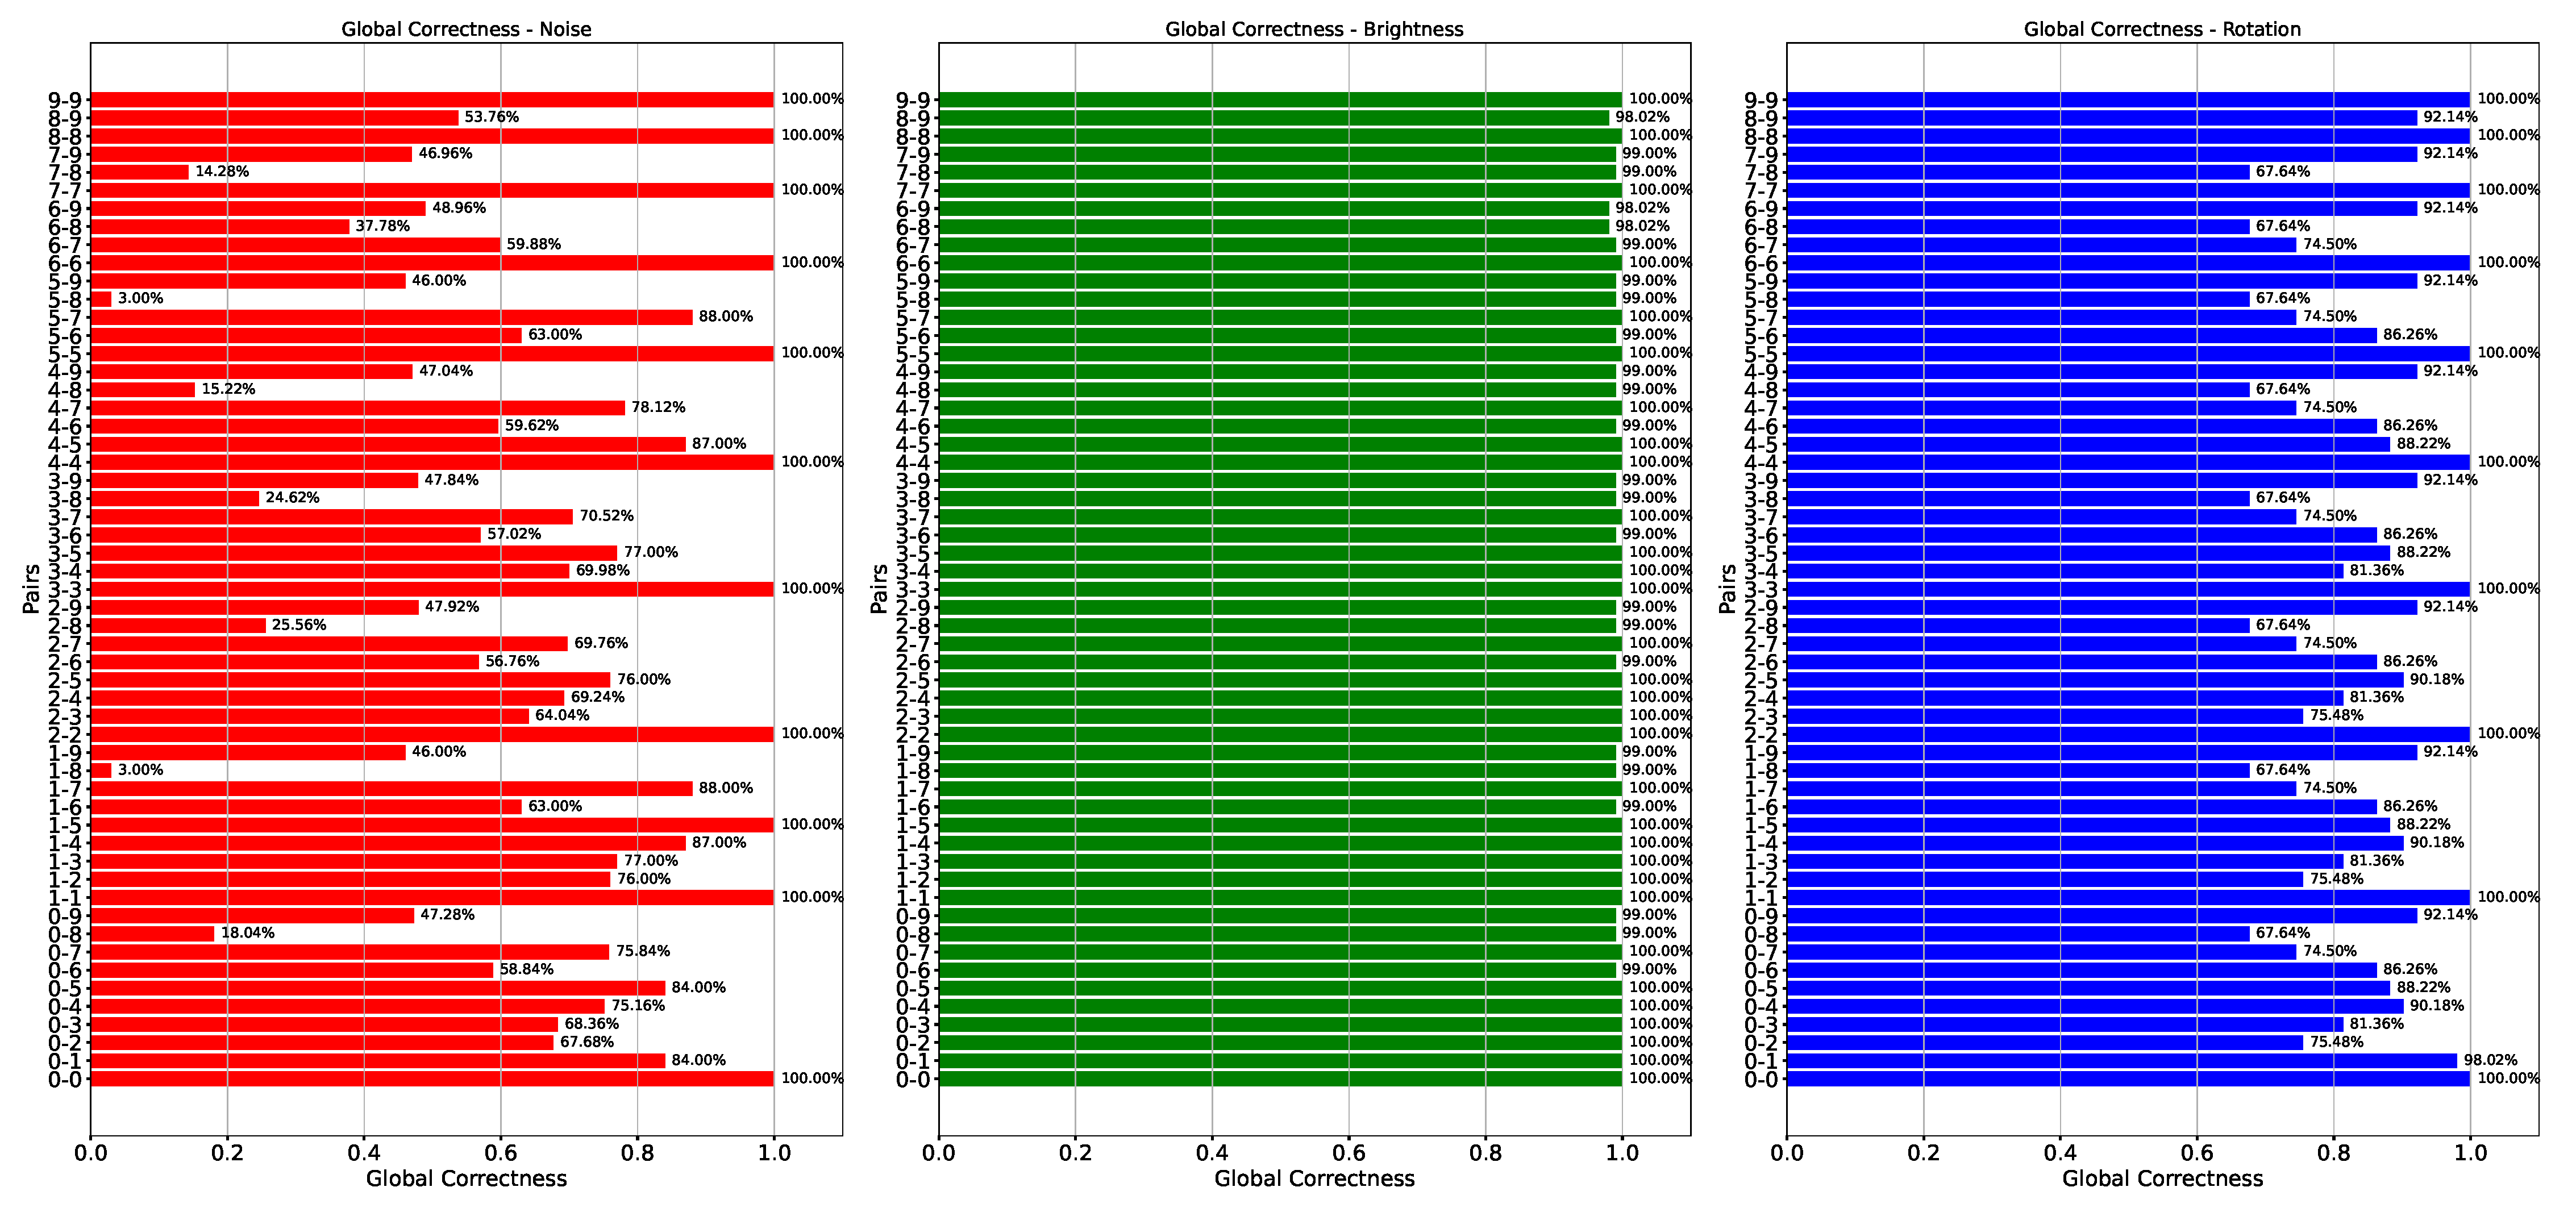
\includegraphics[width=\textwidth]{global_correctness.eps}
    \caption{Global Correctness for Noise, Brightness, and Rotation Transformations}
    \label{fig:global_correctness}
\end{figure}

\begin{figure}[H]
    \centering
    \includegraphics[width=0.8\textwidth]{global_correctness_combine.eps}
    \caption{Final Global Correctness}
    \label{fig:final_global_correctness}
\end{figure}

The global correctness values for pairs of digits under the noise transformation vary significantly. Some pairs such as (0,0), (1,1), (2,2), etc., achieve perfect correctness (100\%), while others like (0,5) and (1,8) exhibit very low correctness (3.00\% and 18.04\%, respectively). This indicates that the model's performance is highly inconsistent under noise, likely due to the distortion introduced affecting digit recognition. The model performs exceptionally well under brightness adjustments, with most pairs achieving near-perfect correctness. This suggests that the model is robust to changes in brightness, maintaining high confidence scores despite variations in image illumination. Performance under rotation is moderate, with significant variations across different pairs. Some pairs like (0,0), (1,1), (3,3), etc., achieve high correctness, while others such as (2,5) and (5,8) have lower correctness values. This variation suggests that while the model can handle certain rotations well, it struggles with others, potentially due to the angles and the inherent difficulty in recognizing rotated digits.

Combining the global correctness across all transformations, we observe an overall high performance with a final global correctness of 97.65\%. **Brightness** contributes the most to this high score (97.03\%), while Noise contributes the least (0.58\%). Rotation has a moderate impact (20.41\%), reflecting its varied performance across different pairs. These observations highlight the strengths and weaknesses of the AI subsystem under different transformations. The high performance under brightness adjustments indicates robustness to illumination changes, while the challenges with noise and rotation suggest areas for improvement in handling these perturbations.


\section{Use Case 2: Autonomous Vehicle Perception}

In this use case, we investigate the robustness of an AI system for autonomous vehicles in detecting objects, particularly vehicles, under various weather conditions including fog, rain, snow, and sand. The goal is to assess the system's performance across these challenging environments to ensure reliable operation.

The dataset was split into training and validation sets, with class balancing performed through oversampling to address any class imbalances. Data augmentation techniques such as rotation, width and height shifts, shear transformation, zoom, and horizontal flips were applied to the training set to enhance the model's generalizability.

The trained model's performance was evaluated on a balanced validation set resampled to ensure uniform class distribution.

\subsection{Local Correctness Analysis}

The local correctness of the model for each weather condition is depicted in the first graph. The AI system exhibits the following correctness values:
- \textbf{Fog:} The detection correctness is 51\%, indicating moderate performance. Fog conditions likely introduce significant visual obstructions that challenge the model's ability to correctly identify vehicles.
- \textbf{Rain:} Achieving a correctness of 75\%, the model performs relatively well in rainy conditions, suggesting robustness to moderate visual disturbances caused by rain.
- \textbf{Snow:} Similar to rain, the system shows a correctness of 75\%, demonstrating its capability to handle snowy environments, where the visual contrast might be reduced.
- \textbf{Sand:} With the highest correctness of 88\%, the model excels in sandy conditions, possibly due to clearer visibility compared to other adverse weather scenarios.

\subsection{Global Correctness Analysis}

\subsection{Global Correctness Evaluation for Vehicle Detection}

The second graph illustrates the global correctness for vehicle detection under different combination methods of weather conditions:

\scalebox{0.9}{%
\begin{minipage}{\linewidth}
\begin{align*}
  global\_weather &\leftrightarrow (fog \land rain \land snow \land sand) \\
  global\_weather &\leftrightarrow (fog \lor rain \lor snow \lor sand) \\
  global\_weather &\leftrightarrow (fog \land (rain \lor snow \lor sand))
\end{align*}
\end{minipage}
}

\begin{figure}[h]
  \centering
  \includegraphics[width=0.8\textwidth]{globalcorrectness_vehicle_detection.eps}
  \caption{Local and Global Correctness of Vehicle Detection Under Various Weather Conditions}
  \label{fig:global_correctness_vehicle_detection}
\end{figure}




\begin{itemize}
    \item \textbf{AND (Intersection):} The model's correctness is 25\%. This low value reflects the stringent requirement for the system to correctly detect vehicles under all specified conditions simultaneously, highlighting potential vulnerabilities when multiple weather challenges are present.
    \item \textbf{OR (Union):} Achieving a perfect correctness of 100\%, the model successfully detects vehicles under at least one of the conditions. This high performance underscores the system's reliability when at least one favorable condition is present.
    \item \textbf{Combination of AND/OR:} The correctness stands at 51\%, representing a balanced approach where the model must correctly detect vehicles under fog and any one of the other conditions (rain, snow, or sand). This mixed strategy provides a realistic measure of the system's robustness in practical scenarios with varying weather conditions.
\end{itemize}



\newpage

%results


% Adjusting chapter title format for regular (numbered) chapters
\titleformat{\chapter}[display]
  {\normalfont\huge\bfseries\centering}{\chaptertitlename\ \thechapter}{20pt}{\Huge}

% Using similar styling for unnumbered chapters but without "Chapter" prefix
\titleformat{name=\chapter,numberless}
  {\normalfont\huge\bfseries\centering}{}{0pt}{\Huge}

\titlespacing*{\chapter}{0pt}{50pt}{40pt} % Adjust vertical spacing before and after the title

\definecolor{barblue}{RGB}{153,204,254}
\definecolor{groupblue}{RGB}{51,102,254}
\definecolor{linkred}{RGB}{165,0,33}
\chapter{PhD Two-Year Plan} % Ensures chapter numbering starts correctly
\label{chp:9}

\section{Research Modules}
I have categorized my research into seven modules as depicted in Figure \ref{fig:no_publish}: Module 1 (DNN Testing Framework), Module 2 (Specification), Module 3 (Sampling), Module 4 (Interpretability), Module 5 (Testcase Generation), Module 6 (Coverage Criteria), and Module 7 (Error Summarization).

\begin{figure}[ht]
  \centering
  \includegraphics[width=\linewidth]{researchareas.png}
  \caption{Research Modules}
  \label{fig:no_publish}
\end{figure}

\section{Mapping of Research Modules to Objectives}
The research is structured into seven distinct modules, each addressing a specific objective. Table \ref{table:modules} outlines the mapping of these research modules to their corresponding objectives discussed in Section \ref{Research Questions and Objectives}.

\begin{table}[ht]
  \centering
  \renewcommand{\arraystretch}{1.5} % Adjusts the row padding
  \begin{tabular}{|l|l|}
    \hline
    \rowcolor[HTML]{000000} 
    \multicolumn{1}{|c|}{\cellcolor[HTML]{000000}{\color[HTML]{FFFFFF} \textbf{Research Modules}}} & {\color[HTML]{FFFFFF} \textbf{Research Objectives}} \\ \hline
    {\color[HTML]{404040} DNN Testing Framework} & Obj1 \\ \hline
    {\color[HTML]{404040} Specification} & Obj2 \\ \hline
    {\color[HTML]{404040} Sampling} & Obj3 \\ \hline
    {\color[HTML]{404040} Interpretability} & Obj4 \\ \hline
    {\color[HTML]{404040} Testcase Generation} & Obj5 \\ \hline
    {\color[HTML]{404040} Coverage Criteria} & Obj6 \\ \hline
    Error Summarization & Obj7 \\ \hline
  \end{tabular}
  \caption{Mapping of Research Modules to Objectives}
  \label{table:modules}
\end{table}

These modules are further divided into specific tasks to streamline the research process:

\subsection{DNN Testing Framework (Module 1, M\textsubscript{Oct24} - M\textsubscript{Sep25}, 43\% completion)} \noindent This module focuses on developing a comprehensive testing framework for DNNs. So far, 43\% of the work is done, including designing the framework, identifying key components, and implementing methods like adversarial and semantic adversarial testcase generation. Previous methods, such as resampling and testcase generation is combined with new solutions like local and global coverage to create a functional pipeline. Next year, I will refine and integrate all components to complete the framework. I have divided it into subtasks. Let's discuss each one in detail.

\noindent \textbf{5.2.1.1 Literature review (M\textsubscript{Oct24} - M\textsubscript{Dec24}, 50\% completion)}\ I have reviewed 50\% of existing DNN testing methods and identified key requirements. Moving forward, I will continue to outline comprehensive testing needs based on further findings.

\noindent \textbf{5.2.1.2 Designing a conceptual framework (M\textsubscript{Oct24} - M\textsubscript{Nov24}, 80\% completion)}\ I have designed 80\% of the framework. I will automate the remaining 20\% of the framework flow according to specified requirements, starting in October 2024.

\noindent \textbf{5.2.1.3 Design local and global coverage flow (M\textsubscript{Oct24} - M\textsubscript{Dec24}, 80\% completion)}\ The design of the local and global coverage flow is 80\% complete. I will focus on gaining more proficiency in running multiple scenarios, models, and datasets, and implementing existing coverage metrics to validate my local and global coverage concept.

\noindent \textbf{5.2.1.4 Implementing the simple real life example to calculate local to global robustness (M\textsubscript{Oct24} - M\textsubscript{Nov24}, 70\% completion)}\ Implemented a simple real-life example to calculate local to global robustness, reaching 70\% completion. The remaining work involves running this example on different DNNs to test effectiveness and further validate the approach.

\noindent \textbf{5.2.1.5 Implement probabilistic logic programming to calculate global coverage with simple examples (M\textsubscript{Oct24} - M\textsubscript{Nov24}, 80\% completion)}\ Set clear criteria for calculating the global coverage. Successfully implemented ProbLog by running a few simple examples, such as an adder and detecting different weather conditions by assuming specifications. These examples were successfully executed using ProbLog. In the coming months, I will run more complex scenarios and datasets related to autonomous driving cars.

\noindent \textbf{5.2.1.6 Integrate probLog code with python code (M\textsubscript{Oct24} - M\textsubscript{Dec24}, 80\% completion)}\ I successfully integrated ProbLog syntax with Python for simple scenarios. In the future, I will focus on integrating it with more complex scenarios and optimizing the code for these complex scenarios.

\noindent \textbf{5.2.1.7 Apply framework to different datasets (M\textsubscript{Oct24} - M\textsubscript{Jun25}, 50\% completion)}\ I have applied the framework, which includes both existing and my proposed components, to the CIFAR, MNIST, and DAWN datasets, reaching 50\% completion. In the future, I will move to more complex datasets, such as those related to autonomous vehicles and other advanced scenarios.

\noindent \textbf{5.2.1.8 Implement existing criteria and integrate proposed coverage criteria (M\textsubscript{Nov24} - M\textsubscript{Jan25}, 40\% completion)}\ I have implemented proposed coverage criteria (local and global) on simple examples, reaching 40\% completion. In the future, I will also implement existing criteria to compare and validate the results of my proposed criteria.

\noindent \textbf{5.2.1.9 Implement and integrate test cases (M\textsubscript{Dec24} - M\textsubscript{March25}, 42\% completion)}\ Implemented various adversarial examples from literature, such as FGSM, BIM and DeepFool, etc., using Foolbox and Adversarial Toolbox library. Additionally, I have implemented semantic adversarial examples like rotation, brightness, noise, and blur using Python code, 42\% is completed. In the future, I will focus on automating these processes and integrating this module into the framework.

\noindent \textbf{5.2.1.10 Implement and integrate interpretability analysis to identify critical features (M\textsubscript{Oct24} - M\textsubscript{Dec24}, 42\% completion)}\ I have explored and applied interpretability techniques, specifically SHAP, to identify critical features in CIFAR and MNIST datasets, reaching 42\% completion. This approach is unique as most research focuses on using these techniques for defensive mechanisms against adversarial examples. In the future, I will explore additional interpretability techniques like LIME and investigate how to better utilize them for my framework, as interpretability is a vast domain with significant potential for enhancing my study.

\noindent \textbf{5.2.1.11 Develop and integrate efficient sampling approach (M\textsubscript{Jan25} - M\textsubscript{Mar25}, 40\% completion)}\ I have read several sampling techniques that are not commonly used by researchers for testing DNNs. I have identified techniques like Borderline SMOTE and ADASYN for finding and prioritize the corner cases, which are not typically used for this purpose in the literature. In the future, I will apply these techniques and develop improved methods for efficient sampling to identify more corner cases.

\noindent \textbf{5.2.1.12 Develop and integrate error summarization modules (M\textsubscript{June25} - M\textsubscript{Aug25}, 0\% completion)}\ I found no existing literature on this component. I have planned to develop a new method for detailed error summarization. This part has not been started yet and will be addressed at the end after implementing all other components.

\noindent \textbf{5.2.1.13 Integrate all developed techniques (M\textsubscript{Aug25} - M\textsubscript{Sep25}, 0\% completion)}\ After working on individual components, I will integrate all components to work automatically within the framework. I will also apply existing methods of different literature papers to validate my proposed framework.


\noindent \textbf{5.2.1.14 Generate results on different datasets and make scenarios to validate this framework (M\textsubscript{Aug25} - M\textsubscript{Sep25}, 35\% completion)}\ Currently working with CIFAR, DAWN, and MNIST datasets, reaching 35\% completion. In the future, I will work with more datasets to further validate the framework.


\subsection{Specification (Module 2, M\textsubscript{Jan25} - M\textsubscript{May25}, 0\% completion)} I have not yet addressed this module in terms of literature or practical work. I tried to find relevant papers, but no significant work focuses on this area. Currently, I assume specifications based on user requirements and perform experiments. In the future, I will automate this part to align the framework with user requirements. I divided this module into subtasks. Let's discuss each one.


\noindent \textbf{5.2.2.1 Read literature about how specification is specified in other systems (M\textsubscript{Jan25} - M\textsubscript{Apr25}, 0\% completion)}\ I plan to work on this in Jan25, after implementing other components of framework. This task will involve reading literature about how specifications are specified in other systems.

\noindent \textbf{5.2.2.2 Find a way to define specification (M\textsubscript{Mar25} - M\textsubscript{Apr25}, 0\% completion)}\ I plan to work on this from Mar25 to Apr25. I will investigate how specifications are defined in other systems, whether they use templates or specific criteria. Additionally, I will determine if I need a template or criteria to define specifications, and how users should provide these, whether in raw form or a specific format.

\noindent \textbf{5.2.2.3 How to pass specifications to ProbLog (M\textsubscript{Apr25} - M\textsubscript{May25}, 0\% completion)}\ I will explore methods to efficiently pass specifications to ProbLog. This includes examin the required format and steps needed for integration between the defined specifications and the ProbLog system.

\noindent \textbf{5.2.2.4 How to automatically change specifications into desired format of framework (M\textsubscript{Apr25} - M\textsubscript{May25}, 0\% completion)}\ I will work on automating the conversion of specifications into the desired format for the framework. This task involves developing a method to transform user-provided specifications into a format compatible with the proposed framework.



\subsection{Sampling (Module 3, M\textsubscript{Jan25} - M\textsubscript{Mar25}, 40\% completion)} Currently, I have achieved 40\% completion by implementing existing sampling techniques specifically for DNN testing. However, I have not explored these techniques in detail. The detailed examination is still pending. So far, I have only implemented these techniques to determine their feasibility, as there is limited research in this area. The module have been separated into subtasks. Let's go through them individually.

\noindent \textbf{5.2.3.1 Reading papers related to sampling techniques and identify gaps (M\textsubscript{Jan25} - M\textsubscript{Feb25}, 50\% completion)}\  I will read various papers related to sampling techniques and identify gaps and potential areas for improvement. This task is already 50\% complete, covering initial literature review and gap identification.

\noindent \textbf{5.2.3.2 Develop efficient sampling technique (M\textsubscript{Feb25} - M\textsubscript{Feb25}, 0\% completion)}\ After identifying gaps in existing techniques, I will develop my own efficient sampling technique specifically for DNN testing. This task aims to create methods that can identify corner cases and enhance overall sampling efficiency.

\noindent \textbf{5.2.3.3 Implement existing sampling techniques (M\textsubscript{Mar25} - M\textsubscript{Mar25}, 70\% completion)}\ I will implement existing sampling techniques, which is already 70\% complete. This involves further testing of these techniques to ensure they are effective for DNN testing.

\noindent \textbf{5.2.3.4 Automate sample generation according to specification (M\textsubscript{Mar25} - M\textsubscript{Mar25}, 0\% completion)}\ I will work on automating the sample generation process according to specified criteria. This task aims to create an efficient method for generating samples that meet the defined specifications.

\subsection{Interpretability (Module 4, M\textsubscript{Oct24} - M\textsubscript{Dec24}, 42\% completion)} This module focuses on applying interpretability techniques to DNNs. Currently, I have achieved 42\% completion by implementing specific methods like SHAP to identify critical features in datasets such as CIFAR and MNIST. Future work will include exploring additional interpretability techniques and further integrating these methods into the framework. Ihave organized it into subtasks. Let's delve into each one specifically.

\noindent \textbf{5.2.4.1 Literature review (M\textsubscript{Oct24} - M\textsubscript{Nov24}, 30\% completion)}\  I will conduct a literature review on interpretability techniques for DNNs. Specifically, I will focus on how to use these techniques to identify critical pixels for effective test case generation, an area that has not been widely explored.

\noindent \textbf{5.2.4.2 Implement SHAP tool (M\textsubscript{Oct24} - M\textsubscript{Nov24}, 100\% completion)}\ Successfully implemented the SHAP tool to identify critical features in DNNs. This task is 100\% complete, providing insights into which pixels are most important for generating effective test cases.

\noindent \textbf{5.2.4.3 Apply SHAP to identify important pixels (M\textsubscript{Oct24} - M\textsubscript{Nov24}, 80\% completion)}\ I have applied the SHAP tool to identify important pixels in DNNs, reaching 80\% completion. In the future, I will apply this technique to different scenarios and datasets to further validate its effectiveness.


\noindent \textbf{5.2.4.4 Explore other interpretability analysis techniques (M\textsubscript{Oct24} - M\textsubscript{Nov24}, 0\% completion)}\ I will explore other interpretability techniques, such as LIME, to identify key features that can guide the generation of optimal test cases for evaluating model robustness. This task is scheduled from M\textsubscript{Oct24} - M\textsubscript{Nov24}, with 0\% completion currently.


\noindent \textbf{5.2.4.5 Automate interpretability approach in test case generation module (M\textsubscript{Nov24} - M\textsubscript{Dec24}, 0\% completion)}\  I will automate the interpretability approach in the test case generation module. This task aims to integrate advanced interpretability techniques to identify critical features in the dataset, which will be used to create effective test cases.

\subsection{Testcase Generation (Module 5, M\textsubscript{Dec24} - M\textsubscript{Mar25}, 42\% completion)} This module focuses on generating test cases for DNNs. Currently, I have achieved 42\% completion by implementing various adversarial and semantic test case generation techniques. Future work will involve automating these processes and integrating them into the overall framework. The module is divided into subtasks. Let's review each one in detail

\noindent \textbf{5.2.5.1 Literature review (M\textsubscript{Dec24} - M\textsubscript{Feb25}, 50\% completion)}\ Conducted a literature review on test case generation techniques for DNNs, reaching 50\% completion. This task covered the period from M\textsubscript{1} to M\textsubscript{18}, identifying key methods and gaps in the current research.

\noindent \textbf{5.2.5.2 Exploring libraries for test case generation (M\textsubscript{Dec24} - M\textsubscript{Jan25}, 80\% completion)}\ Explored various libraries for test case generation, reaching 80\% completion. This involved evaluating tools and frameworks that can be utilized for generating test cases for DNNs.

\noindent \textbf{5.2.5.3 Implementing adversarial attacks and semantic adversarial test cases (M\textsubscript{Dec24} - M\textsubscript{Dec24}, 80\% completion)}\ I have implemented adversarial attacks and semantic adversarial test cases, reaching 80\% completion. This involved creating test cases that simulate real-world adversarial scenarios and environmental variations to evaluate the robustness of DNNs.

\noindent \textbf{5.2.5.4 Apply existing test case generation methods to benchmark datasets (M\textsubscript{Jan25} - M\textsubscript{Feb25}, 0\% completion)}\ I will apply existing test case generation methods to benchmark datasets and analyze the results. This task is scheduled from M\textsubscript{13} to M\textsubscript{14}, with 0\% completion currently.

\noindent \textbf{5.2.5.5 Automate proposed test generation module (M\textsubscript{Feb25} - M\textsubscript{Mar25}, 0\% completion)}\ From Feb25 to Mar25, I will work on automating the proposed test generation module. This task aims to develop a seamless and efficient process for generating test cases automatically based on the proposed methods.

\subsection{Coverage Criteria (Module 6, M\textsubscript{Nov24} - M\textsubscript{Jan25}, 40\% completion)} This module focuses on developing and implementing coverage criteria for DNN testing. Currently, I have achieved 40\% completion by identifying and partially implementing existing coverage criteria. Future work will involve refining these criteria and integrating them into the overall framework. I have broken this module into subtasks. Let's go over each one in detail.


\noindent \textbf{5.2.6.1 Literature review on coverage criteria (M\textsubscript{Nov24} - M\textsubscript{Dec24}, 40\% completion)}\ I have reviewed literature on coverage criteria and found that existing methods often focus on internal structures of DNNs, neglecting comprehensive coverage. I proposed new local and global coverage concepts, designed, and implemented them using CIFAR and MNIST datasets. Future work will focus on refining and applying these criteria to improve DNN testing coverage.


\noindent \textbf{5.2.6.1 Reading papers and identifying gaps (M\textsubscript{Nov24} - M\textsubscript{Dec24}, 80\% completion)}\ I have reviewed relevant literature on coverage criteria and identified that many existing methods focus mainly on the internal structures of DNNs. I proposed new local and global coverage criteria to address these gaps. The work completed includes reviewing the current methods and implementing the proposed criteria using CIFAR and MNIST datasets. Future efforts will be directed towards further development and application of these coverage criteria.


\noindent \textbf{5.2.6.3 Apply existing coverage criteria to benchmark datasets (M\textsubscript{Nov24} - M\textsubscript{Dec24}, 0\% completion)}\ I plan to apply existing coverage criteria to benchmark datasets like CIFAR and MNIST. This task will involve evaluating the effectiveness of these criteria to understand their performance and limitations. The analysis will help determine how well the current methods align with the proposed coverage concepts and provide insights for further refinement.

\noindent \textbf{5.2.6.4 Reading literature on probLog to understand its application in calculating DNN global coverage (M\textsubscript{Dec24} - M\textsubscript{Dec24}, 50\% completion)}\ I will review literature on ProbLog to understand its application for calculating global coverage in DNNs. This review will explore how ProbLog has been used for global coverage analysis, identifying gaps and opportunities for improvement in the context of deep neural networks.


\noindent \textbf{5.2.6.5 Understand the probLog language and editor (M\textsubscript{Nov24} - M\textsubscript{Jan25}, 70\% completion)}\ I have achieved a 70\% understanding of the ProbLog language and its editor, including basic rule definitions and query manipulations. Further efforts will focus on deepening this knowledge and mastering advanced features to effectively implement and refine ProbLog-based solutions for coverage criteria.


\noindent \textbf{5.2.6.6 Implementing and automating probLog for DNN coverage calculations (M\textsubscript{Dec24} - M\textsubscript{Jan25}, 0\% completion)}\ I will implement and automate ProbLog to calculate DNN coverage. This will involve integrating ProbLog with the framework and automating its use to ensure accurate and efficient coverage calculations.

\subsection{Error Summarization (Module 7, M\textsubscript{Jun25} - M\textsubscript{Aug25}, 0\% completion)}This module, starting in June 2025, will focus on developing methods for summarizing errors in DNN testing. It will involve creating a new approach for error analysis and summarization, following the completion of all previous modules. I have split the work into subtasks. Let's discuss them one by one.


\noindent \textbf{5.2.7.1 Find ways to properly summarize the counter examples (M\textsubscript{Jun25} - M\textsubscript{July25}, 0\% completion)}\ I will explore methods to effectively summarize counterexamples in DNN testing. This will involve identifying techniques for detailed error analysis and summarization to enhance understanding and improve the framework's robustness.

\noindent \textbf{5.2.7.2 Best visuals to represent errors report (M\textsubscript{July25} - M\textsubscript{Aug25}, 0\% completion)}\ I will identify and implement effective visualizations to represent error reports. This involves evaluating various visualization techniques to determine which best conveys error patterns and insights, enhancing the clarity and usefulness of error summaries

\noindent \textbf{5.2.7.3 Integrate error summarization module in framework (M\textsubscript{July25} - M\textsubscript{Aug25}, 0\% completion)}\ I will integrate the error summarization module into the existing framework. This will involve ensuring that the module works seamlessly with other components and effectively summarizes errors generated during testing, providing a comprehensive view of model performance and issues.

\section{Mapping of Research Milestones to Objectives}
This section outlines the key milestones in the research timeline.The planned milestones and their associated research objectives are detailed in Table \ref{table:milestones}. This table maps each milestone to the specific objectives it addresses, including major conferences, journal papers, and thesis-related activities.

\noindent \textbf{MS1: Conference 1} \
I will present initial research findings and theoretical contributions at the first conference, focusing on early results and their implications.

\noindent \textbf{MS2: Conference 2} \
I will showcase refined results and new insights at the second conference. This presentation will highlight advancements in methodology and preliminary data analysis.

\noindent \textbf{MS3: Journal 1} \
I will publish a detailed research paper in a peer-reviewed journal, documenting significant findings and contributions to the field.

\noindent \textbf{MS4: Conference 3} \
I will present further research progress and innovations at the third conference, focusing on advanced techniques and expanded data sets.

\noindent \textbf{MS5: Conference 4} \
I will deliver a presentation on the latest developments and comprehensive results at the fourth conference, emphasizing contributions to current research trends.

\noindent \textbf{MS6: Journal 2 } \
I will submit and publish a follow-up paper in a second peer-reviewed journal, detailing additional findings and improvements from recent research.

\noindent \textbf{MS7: Thesis Writing } \
I will draft the thesis, integrating all research milestones, methodologies, and results. This will involve organizing and presenting comprehensive findings.

\noindent \textbf{MS8: Thesis Submission} \
I will submit the finalized thesis to the academic committee for review, incorporating feedback and ensuring that all research objectives and contributions are documented.

\noindent \textbf{MS9: Defense and Final Submission} \
I will prepare for and conduct the thesis defense, make final revisions based on feedback, and submit the final version of the thesis, completing the research project.

\begin{table*}[ht]
  \centering
  \renewcommand{\arraystretch}{1.5} 
  \resizebox{\textwidth}{!}{%
    \begin{tabular}{|l|l|}
      \hline
      \rowcolor[HTML]{000000} 
      \multicolumn{1}{|c|}{\cellcolor[HTML]{000000}{\color[HTML]{FFFFFF} \textbf{Milestones}}} & {\color[HTML]{FFFFFF} \textbf{Research Objectives}} \\ \hline
      {\color[HTML]{404040} Conference 1 (EuroML Conf 2025)} & Obj1, 4, 6 \\ \hline
      {\color[HTML]{404040} Conference 2 (ICSE 2025)} & Obj2 \\ \hline
      {\color[HTML]{404040} Journal paper 1 (Neural Networks)} & Obj1, 2, 4, 6 \\ \hline
      {\color[HTML]{404040} Conference 3 (ASE 2025)} & Obj3 \\ \hline
      {\color[HTML]{404040} Conference 4 (ICST 2025)} & Obj7 \\ \hline
      {\color[HTML]{404040} Journal paper 2 (IEEE Transaction on Software Engineering)} & Obj1, 2, 3, 7 \\ \hline
      {\color[HTML]{404040} Thesis writing} & compile and synthesize research findings  \\ \hline
      {\color[HTML]{404040} Thesis submission} & finalize and submit the complete thesis  \\ \hline
      {\color[HTML]{404040} Defense and final submission} & present research, address feedback, and submit final version\\ \hline
    \end{tabular}
  }
  \caption{Mapping of Research Milestones to Objectives}
  \label{table:milestones}
\end{table*}


\section{Gantt Chart for Task-Wise Completion}
The Gantt chart provides a clear timeline and progress overview for the research project. Modules, such as Module 1 (M1), Module 2 (M2), and Module 3 (M3), are depicted with color-coded bars to indicate their progress. The dark blue bars represent the percentage of work completed within each module, reflecting the overall progress. In contrast, black lines show the completion status for each Module. Tasks following the M1,2,3..7, are represented by blue lines. The sky blue bars indicate the percentage of completion for these tasks, while the light blue bars represent the remaining portion that is still pending. Milestones, such as Conference paper 1 (MS1), are marked with red circles, highlighting key achievements and deadlines. This color-coding effectively communicates the status and progress of various tasks and milestones throughout the project.

\hspace{-3.5cm}
\begin{ganttchart}[
  y unit chart=0.6cm,
  x unit=0.023cm,
  vgrid={*1{draw=none}, *1{draw=black!10}}, % Reduce vertical grid lines
  hgrid={*1{draw=black!20}}, % Reduce horizontal grid lines
  time slot format=isodate,
  title/.append style={fill=none, draw=black},
  title label font=\bfseries\footnotesize\color{black},
  bar/.append style={draw=none, fill=barblue},
  bar incomplete/.append style={fill=barblue!50},
  bar label font=\bfseries\footnotesize\color{black},
  group incomplete/.append style={fill=groupblue},
  group left shift=0,
  group right shift=0,
  group height=.4,
  group peaks tip position=0,
  group label node/.append style={left=.5cm},
  group progress label font=\bfseries\small,
  link/.append style={-latex, line width=1.5pt, linkred},
  link label font=\scriptsize\bfseries,
  link label node/.append style={below left=-2pt and 4pt},
  milestone/.append style={shape=circle, fill=none},
  milestone label font=\bfseries\footnotesize\color{red},
  milestone label node/.append style={left=5mm, above left=-5mm and 0mm}
]{2024-10-01}{2026-11-30}
\gantttitlecalendar{year, month=shortname} \\

% Module 1: DNN Testing Framework
\ganttgroup[progress=43]{M1}{2024-10-01}{2025-9-29} \\
\ganttbar[progress=50]{5.2.1.1}{2024-10-01}{2024-12-28}\\ % Literature review (M1-M5)
\ganttbar[progress=80]{5.2.1.2}{2024-10-01}{2024-11-30}\\ % Designing a conceptual framework (M8-M12)
\ganttbar[progress=80]{5.2.1.3}{2024-10-01}{2024-12-31} \\% Design local and global coverage flow (M8-M10)
\ganttbar[progress=70]{5.2.1.4}{2024-10-01}{2024-11-31}\\ % Implementing the Simple real life Example (M8-M10)
\ganttbar[progress=80]{5.2.1.5}{2024-10-01}{2024-11-30} \\% Implementing ProbLog for calculating global robustness (M9-M11)
\ganttbar[progress=80]{5.2.1.6}{2024-10-01}{2024-12-30} \\% Integrate ProbLog code with python code (M9-M11)
\ganttbar[progress=50]{5.2.1.7}{2024-10-01}{2025-6-31} \\% Applying the framework to different datset
\ganttbar[progress=40]{5.2.1.8}{2024-11-01}{2025-1-30} \\% Implement exisiting criterias and integrate proposed coverage criteria 

\ganttbar[progress=42]{5.2.1.9}{2024-12-01}{2025-3-3} \\% Implement and integrate testcases 
\ganttbar[progress=42]{5.2.1.10}{2024-10-01}{2024-12-31} \\% Implement and integrate interpratability analysis to identofy critical features


% Milestone MS1 with red dot
\ganttmilestone[
  milestone/.append style={shape=circle, fill=red, minimum size=3mm},
  milestone label font=\bfseries\footnotesize\color{black},
  milestone label node/.append style={right=20mm, yshift=0mm}
]{Conference paper 1(MS1)}{2024-12-15}\\

\ganttbar[progress=40]{5.2.1.11}{2025-1-01}{2025-3-30} \\% Develop and integrate efficient sampling approach
\ganttbar[progress=0]{5.2.1.12}{2025-1-01}{2025-5-30} \\% Develop and integrate specifcation templates
\ganttbar[progress=0]{5.2.1.13}{2025-6-01}{2025-8-30} \\% Develop and integrate error summarzation modules
\ganttbar[progress=0]{5.2.1.14}{2025-8-01}{2025-9-30} \\% Integrate all developed techniques
\ganttbar[progress=35]{5.2.1.15}{2025-8-01}{2025-9-10} \\% Generate results on different datasets  and make scenarios to validate this framework.


% Module 2: Specification
\ganttgroup[progress=0]{M2} {2025-01-01}{2025-5-30} \\
\ganttbar[progress=0]{5.2.2.1}{2025-01-01}{2025-04-31} \\% Read literature about how specification specified in other systems
\ganttbar[progress=0]{5.2.2.1}{2025-03-01}{2025-04-31} \\% Find a way to define specification (M20-M23)
\ganttbar[progress=0]{5.2.2.2}{2025-04-01}{2025-05-31} \\% How to pass specifications to ProbLog (M20-M23)
\ganttbar[progress=0]{5.2.2.3}{2025-04-01}{2025-05-1}\\ % How to automatically change specifications into desired format of framework

% \ganttmilestone{MS2}{2025-05-30}\\

% \ganttmilestone[inline]{\tikz \node[shape=circle, fill=red, minimum size=3mm, inner sep=0pt] {};\ MS1}{2025-05-30}\\

\ganttmilestone[
  milestone/.append style={shape=circle, fill=red, minimum size=3mm},
  milestone label font=\bfseries\footnotesize\color{black},
  milestone label node/.append style={right=60mm, yshift=0mm}
]{Conference paper 2(MS2)}{2025-05-30}\\

\ganttmilestone[
  milestone/.append style={shape=circle, fill=red, minimum size=3mm},
  milestone label font=\bfseries\footnotesize\color{black},
  milestone label node/.append style={right=29mm, yshift=0mm}
]{Journal paper 1(MS3)}{2025-1-30}\\

  % % Module 3: Sampling

% \ganttmilestone{MS4}{2025-1-30}\\
\ganttgroup[progress=40]{M3}{2025-1-1}{2025-03-30} \\
\ganttbar[progress=50]{5.2.3.1}{2025-1-1}{2025-02-15}\\ % Reading Papers Related to Sampling Techniques and Identify Gaps (M9-M10)
\ganttbar[progress=0]{5.2.3.2}{2025-2-15}{2025-02-30} \\% Develop Efficient Sampling Technique (M10-M12)
\ganttbar[progress=70]{5.2.3.3}{2025-3-01}{2025-3-10} \\% Implement Existing Sampling Techniques (M9-M10)
\ganttbar[progress=0]{5.2.3.4}{2025-3-01}{2025-03-30} \\% Automate sampling according to specification
% \ganttmilestone{MS4}{2025-3-15}\\
\ganttmilestone[
  milestone/.append style={shape=circle, fill=red, minimum size=3mm},
  milestone label font=\bfseries\footnotesize\color{black},
  milestone label node/.append style={right=40mm, yshift=0mm}
]{Conference paper 3(MS4)}{2025-3-15}\\


\end{ganttchart}
\newpage
\hspace{-3.5cm}
\begin{ganttchart}[
  y unit chart=0.6cm,
  x unit=0.023cm,
  vgrid={*1{draw=none}, *1{draw=black!10}}, % Reduce vertical grid lines
  hgrid={*1{draw=black!20}}, % Reduce horizontal grid lines
  time slot format=isodate,
  title/.append style={fill=none, draw=black},
  title label font=\bfseries\footnotesize\color{black},
  bar/.append style={draw=none, fill=barblue},
  bar incomplete/.append style={fill=barblue!50},
  bar label font=\bfseries\footnotesize\color{black},
  group incomplete/.append style={fill=groupblue},
  group left shift=0,
  group right shift=0,
  group height=.4,
  group peaks tip position=0,
  group label node/.append style={left=.5cm},
  group progress label font=\bfseries\small,
  link/.append style={-latex, line width=1.5pt, linkred},
  link label font=\scriptsize\bfseries,
  link label node/.append style={below left=-2pt and 0pt},
  milestone/.append style={shape=circle, fill=red, minimum size=5mm},
  milestone label font=\bfseries\footnotesize\color{red},
  milestone label node/.append style={left=5mm, above left=-5mm and 0mm}
]{2024-10-01}{2026-11-30}
  \gantttitlecalendar{year, month=shortname} \\


  % % Module 4: Interpretability 2024-10-01}{2024-12-31}
  \ganttgroup[progress=42]{M4}{2024-10-01}{2024-12-31} \\
  \ganttbar[progress=30]{5.2.4.1}{2024-10-01}{2024-11-30}\\ % Literature Review (M4-M24)
  \ganttbar[progress=100]{5.2.4.2}{2024-10-01}{2024-11-31}\\ % Implementation of SHAP Tool (M4-M6)
  \ganttbar[progress=80]{5.2.4.3}{2024-10-01}{2024-11-31}\\ % Applying SHAP to Identify Important Pixels (M4-M5)
  \ganttbar[progress=0]{5.2.4.4}{2024-10-15}{2024-11-30}\\ % Explore Other Interpretability Analysis Techniques (M15-M17)
  \ganttbar[progress=0]{5.2.4.5}{2024-11-01}{2024-12-30}\\ 
  % Automate Interpretability Approach in Test Case Generation Module (M16-M17)



% Module 5: Testcase Generation {2024-12-01}{2025-3-3} 
\ganttgroup[progress=42]{M5}{2024-12-01}{2025-03-03} \\
\ganttbar[progress=50]{5.2.5.1}{2024-12-01}{2025-02-31}\\ % Literature Review (M1-M18)
\ganttbar[progress=80]{5.2.5.2}{2024-12-01}{2025-01-1}\\ % Exploring Libraries for Test Case Generation (M1-M2)
\ganttbar[progress=80]{5.2.5.3}{2024-12-01}{2024-12-31}\\ % Implementing Adversarial Attacks and Semantic Adversarial Test Cases (M3-M4)
\ganttbar[progress=0]{5.2.5.4}{2025-1-01}{2025-02-30}\\ % Apply Existing Test Case Generation Methods to Benchmark Datasets (M13-M14)
\ganttbar[progress=0]{5.2.5.5}{2025-2-01}{2025-03-30}\\ % Automate Proposed Test Generation Module (M15-M16)

% Module 6: Coverage Criteria {2024-11-01}{2025-1-30} 
\ganttgroup[progress=40]{M6}{2024-11-01}{2025-1-30} \\
\ganttbar[progress=80]{5.2.6.1}{2024-11-01}{2024-12-1}\\ % Reading Papers and Identifying Gaps (M6-M9)
\ganttbar[progress=0]{5.2.6.2}{2024-11-01}{2024-12-30}\\ % Apply Existing Coverage Criteria to Benchmark Datasets (M13-M14)
\ganttbar[progress=50]{5.2.6.3}{2024-12-01}{2024-12-31}\\ % Reading Literature on ProbLog to Understand its Application in Calculating DNN Global Coverage

\ganttbar[progress=70]{5.2.6.4}{2024-11-01}{2025-1-30} \\% Understand the Problog Language and Editor (M9-M10)
\ganttbar[progress=0]{5.2.6.5}{2024-12-01}{2025-1-30}\\ % Implementing and Automating ProbLog for DNN Coverage Calculations


% Module 7: Error Summarization {2025-6-01}{2025-8-30}
\ganttgroup[progress=0]{M7}{2025-6-01}{2025-08-30} \\
\ganttbar[progress=0]{5.2.7.1}{2025-06-01}{2025-07-31}\\ % Find Ways to Properly Summarize the Counter Examples (M17-M18)
\ganttbar[progress=0]{5.2.7.2}{2025-7-01}{2025-08-30} \\% Best Visuals to Represent Errors Report (M18-M20)
\ganttbar[progress=0]{5.2.7.3}{2025-7-01}{2025-08-30}\\ % Integrate Error Summarization Module in Framework (M20-M21)

\ganttmilestone[
  milestone/.append style={shape=circle, fill=red, minimum size=3mm},
  milestone label font=\bfseries\footnotesize\color{black},
  milestone label node/.append style={right=120mm, yshift=0mm}
]{Conference paper 4(MS5)}{2026-02-30}\\

\ganttmilestone[
  milestone/.append style={shape=circle, fill=red, minimum size=3mm},
  milestone label font=\bfseries\footnotesize\color{black},
  milestone label node/.append style={right=143mm, yshift=0mm}
]{Journal paper 2(MS6)}{2026-06-1}\\


% \ganttmilestone{MS5}{2025-08-30}\\
% \ganttmilestone{MS4}{2025-09-1}\\

% \ganttbar[progress=20]{\textcolor{red}{MS7}}{2024-10-01}{2026-05-30} \\
 \ganttbar[progress=20]{MS7}{2024-10-01}{2026-05-30} \\
\ganttmilestone[
  milestone/.append style={shape=circle, fill=red, minimum size=3mm},
  milestone label font=\bfseries\footnotesize\color{black},
  milestone label node/.append style={right=110mm, yshift=0mm}
]{Thesis submission(MS8)}{2026-7-30}\\
\ganttmilestone[
  milestone/.append style={shape=circle, fill=red, minimum size=3mm},
  milestone label font=\bfseries\footnotesize\color{black},
  milestone label node/.append style={right=112mm, yshift=0mm}
]{Defense and final submission(MS9)}{2026-10-30}\\


% \ganttmilestone{MS8}{2026-7-30}\\
% % \ganttbar[progress=0]{MS9}{2026-7-01}{2026-10-30} \\
% \ganttmilestone{MS9}{2026-10-30}\\
\end{ganttchart}
% \end{landscape}
% }

% \chapter{References} % Ensures chapter numbering starts correctly
% Adjusting chapter title format for regular (numbered) chapters
\titleformat{\chapter}[display]
  {\normalfont\huge\bfseries\centering}{\chaptertitlename\ \thechapter}{20pt}{\Huge}

% Using similar styling for unnumbered chapters but without "Chapter" prefix
\titleformat{name=\chapter,numberless}
  {\normalfont\huge\bfseries\centering}{}{0pt}{\Huge}

\titlespacing*{\chapter}{0pt}{50pt}{40pt} % Adjust vertical spacing before and after the title


\label{chp:5}
\begin{singlespace}
\begin{thebibliography}{}

% BACKGROUND

\bibitem{ZhaoXBanks}Zhao, X., Banks, A., Sharp, J., Robu, V., Flynn, D., Fisher, M., and Huang, X. (2020). A safety framework for critical systems utilising deep neural networks. In Computer Safety, Reliability, and Security: 39th International Conference, SAFECOMP 2020, Lisbon, Portugal, September 16–18, 2020, Proceedings 39 (pp. 244-259). Springer International Publishing.


\bibitem{LeCun}LeCun, Y., Bengio, Y. and Hinton, G., 2015. Deep learning. nature, 521(7553), pp.436-444.

\bibitem{HuangX}Huang, X., Kroening, D., Ruan, W., Sharp, J., Sun, Y., Thamo, E., Wu, M. and Yi, X., 2020. A survey of safety and trustworthiness of deep neural networks: Verification, testing, adversarial attack and defence, and interpretability. Computer Science Review, 37, p.100270.

% robustness and correctness 

\bibitem{Goodfellow} Goodfellow, I. J., Shlens, J., \& Szegedy, C. (2015). Explaining and Harnessing Adversarial Examples. In Proceedings of the International Conference on Learning Representations (ICLR). Link to Paper

\bibitem{Carlini} Carlini, N., \& Wagner, D. (2017). Towards Evaluating the Robustness of Neural Networks. In Proceedings of the IEEE Symposium on Security and Privacy (SP).
   
\bibitem{Sekhon} Sekhon, Jasmine, and Cody Fleming. "Towards improved testing for deep learning." 2019 IEEE/ACM 41st International Conference on Software Engineering: New Ideas and Emerging Results (ICSE-NIER). IEEE, 2019.

\bibitem{Rushby}Rushby, J. (2015). The interpretation and evaluation of assurance cases. Technical report, SRI International.

%LITERATURE





 \bibitem{dnn_archi}Liu, W., Wang, Z., Liu, X., Zeng, N., Liu, Y. and Alsaadi, F.E., 2017. A survey of deep neural network architectures and their applications. Neurocomputing, 234, pp.11-26.    \bibitem{Hassija}Hassija, V., Chamola, V., Mahapatra, A., Singal, A., Goel, D., Huang, K., Scardapane, S., Spinelli, I., Mahmud, M. and Hussain, A., 2024. Interpreting black-box models: a review on explainable artificial intelligence. Cognitive Computation, 16(1), pp.45-74.
 \bibitem{Liang}Liang, Y., Li, S., Yan, C., Li, M. and Jiang, C., 2021. Explaining the black-box model: A survey of local interpretation methods for deep neural networks. Neurocomputing, 419, pp.168-182.
   
\bibitem{Hosseini}
Hosseini, H. and Poovendran, R., 2018. Semantic adversarial examples. In Proceedings of the IEEE Conference on Computer Vision and Pattern Recognition Workshops (pp. 1614-1619).

\bibitem{adv_attacks}Ren, K., Zheng, T., Qin, Z. and Liu, X., 2020. Adversarial attacks and defenses in deep learning. Engineering, 6(3), pp.346-360.

\bibitem{deeptest}Tian, Y., Pei, K., Jana, S. and Ray, B., 2018, May. Deeptest: Automated testing of deep-neural-network-driven autonomous cars. In Proceedings of the 40th international conference on software engineering (pp. 303-314).


% sampling
    \bibitem{Frey1997} Frey, B. J., \& Fisher, D. H. (1997). Modeling Decision Tree Performance with the Power Law. In \textit{Proceedings of the Fourteenth International Conference on Machine Learning} (pp. 59-65).
    \bibitem{Katz2017} Katz, G., Barrett, C., Dill, D. L., Julian, K., \& Kochenderfer, M. J. (2017). Reluplex: An Efficient SMT Solver for Verifying Deep Neural Networks. In \textit{Proceedings of the 29th International Conference on Computer Aided Verification} (pp. 97-117).
    \bibitem{Chawla2002} Chawla, N. V., Bowyer, K. W., Hall, L. O., \& Kegelmeyer, W. P. (2002). SMOTE: Synthetic Minority Over-sampling Technique. \textit{Journal of Artificial Intelligence Research}, 16, 321-357.
    \bibitem{He2008} He, H., Bai, Y., Garcia, E. A., \& Li, S. (2008). ADASYN: Adaptive Synthetic Sampling Approach for Imbalanced Learning. In \textit{2008 IEEE International Joint Conference on Neural Networks (IEEE World Congress on Computational Intelligence)} (pp. 1322-1328). IEEE.
    \bibitem{Mani2003} Mani, I., \& Zhang, I. (2003). kNN approach to unbalanced data distributions: a case study involving information extraction. In \textit{Proceedings of Workshop on Learning from Imbalanced Datasets} (Vol. 126).
    \bibitem{Han2005} Han, H., Wang, W.-Y., \& Mao, B.-H. (2005). Borderline-SMOTE: A New Over-Sampling Method in Imbalanced Data Sets Learning. In \textit{Advances in Intelligent Computing, ICIC 2005} (pp. 878-887). Springer.
    \bibitem{Roth2019} Roth, K., Kilcher, Y., \& Hofmann, T. (2019). Adversarial Training for Weakly Supervised Learning. In \textit{Advances in Neural Information Processing Systems} (Vol. 32).


   
    
    \bibitem{deepxplore} Pei, K., Cao, Y., Yang, J. and Jana, S., 2017, October. Deepxplore: Automated whitebox testing of deep learning systems. In proceedings of the 26th Symposium on Operating Systems Principles (pp. 1-18).

    \bibitem{deepguage}Ma, L., Juefei-Xu, F., Zhang, F., Sun, J., Xue, M., Li, B., Chen, C., Su, T., Li, L., Liu, Y. and Zhao, J., 2018, September. Deepgauge: Multi-granularity testing criteria for deep learning systems. In Proceedings of the 33rd ACM/IEEE international conference on automated software engineering (pp. 120-131).
    
    \bibitem{SunY}Sun, Y., Huang, X., Kroening, D., Sharp, J., Hill, M. and Ashmore, R., 2018. Testing deep neural networks. arXiv preprint arXiv:1803.04792.

    \bibitem{KimJ}Kim, J., Feldt, R. and Yoo, S., 2019, May. Guiding deep learning system testing using surprise adequacy. In 2019 IEEE/ACM 41st International Conference on Software Engineering (ICSE) (pp. 1039-1049). IEEE.
  
   
    \bibitem{dlfuzz}Guo, J., Jiang, Y., Zhao, Y., Chen, Q. and Sun, J., 2018, October. Dlfuzz: Differential fuzzing testing of deep learning systems. In Proceedings of the 2018 26th ACM Joint Meeting on European Software Engineering Conference and Symposium on the Foundations of Software Engineering (pp. 739-743).

    \bibitem{tensorfuzz} Odena, A., Olsson, C., Andersen, D. and Goodfellow, I., 2019, May. Tensorfuzz: Debugging neural networks with coverage-guided fuzzing. In International Conference on Machine Learning (pp. 4901-4911). PMLR.

    \bibitem{deepconcolic}Sun, Y., Huang, X., Kroening, D., Sharp, J., Hill, M. and Ashmore, R., 2019, May. DeepConcolic: Testing and debugging deep neural networks. In 2019 IEEE/ACM 41st International Conference on Software Engineering: Companion Proceedings (ICSE-Companion) (pp. 111-114). IEEE.


% test and verification
    \bibitem{Albarghouthi}
    Aws Albarghouthi, Introduction to Neural Network Verification,2021.
    
    \bibitem{DeepMind2023}
    DeepMind Safety Research, Towards Robust and Verified AI: Specification Testing, Robust Training, and Formal Verification.

    \bibitem{Urban2021}
    Caterina Urban, et al., A Review of Formal Methods applied to Machine Learning,2021.

    






\bibitem{Agarwal} Agarwal, Aniya, et al. "Automated test generation to detect individual discrimination in AI models." arXiv preprint arXiv:1809.03260 (2018).

\bibitem{Youcheng} Sun, Youcheng, et al. "Concolic testing for deep neural networks." Proceedings of the 33rd ACM/IEEE International Conference on Automated Software Engineering. 2018.

\bibitem{Kexin} Pei, Kexin, et al. "DeepXplore." Communications of the ACM 62.11 (2019): 137-145.

\bibitem{Yuchi} Tian, Yuchi, et al. "Deeptest: Automated testing of deep-neural-network-driven autonomous cars." Proceedings of the 40th international conference on software engineering. 2018.

\bibitem{Sun} Sun, Youcheng, et al. "Testing deep neural networks." arXiv preprint arXiv:1803.04792 (2018).

\bibitem{Ma} Ma, Lei, et al. "Deepgauge: Multi-granularity testing criteria for deep learning systems." Proceedings of the 33rd ACM/IEEE international conference on automated software engineering. 2018.

\bibitem{Zhang} Zhang, Mengshi, et al. "DeepRoad: GAN-based metamorphic testing and input validation framework for autonomous driving systems." Proceedings of the 33rd ACM/IEEE International Conference on Automated Software Engineering. 2018.

\bibitem{Xie} Xie, Xiaofei, et al. "Deephunter: Hunting deep neural network defects via coverage-guided fuzzing." arXiv preprint arXiv:1809.01266 (2018).

\bibitem{Gopinath}	Gopinath, Divya, et al. "Symbolic execution for deep neural networks." arXiv preprint arXiv:1807.10439 (2018).

% \bibitem{DeRaedt}
% De Raedt, L., Kimmig, A. and Toivonen, H., 2007, January. Problog: A probabilistic prolog and its application in link discovery. In IJCAI (Vol. 7, pp. 2462-2467).

% \bibitem{DeepProbLog}
% Manhaeve, R., Dumancic, S., Kimmig, A., Demeester, T. and De Raedt, L., 2018. Deepproblog: Neural probabilistic logic programming. Advances in neural information processing systems, 31.
\bibitem{Sato1997} Sato, T., Kameya, Y.: PRISM: A symbolic-statistical modeling language. In: IJCAI. pp. 1330--1339 (1997)

\bibitem{Koller2009} Koller, D., Friedman, N.: Probabilistic Graphical Models: Principles and Techniques. MIT Press (2009)

\bibitem{Vennekens2004} Vennekens, J., Denecker, M., Bruynooghe, M.: Logic programs with annotated disjunctions. In: ICLP. pp. 195--209 (2004)

\bibitem{DeRaedt2007} De Raedt, L., Kimmig, A., Toivonen, H.: ProbLog: A probabilistic Prolog and its application in link discovery. In: IJCAI. pp. 2462--2467 (2007)

\bibitem{Poole1993} Poole, D.: Probabilistic Horn abduction and Bayesian networks. Artificial Intelligence 64(1), 81--129 (1993)

\bibitem{Poole1997} Poole, D.: The independent choice logic for modelling multiple agents under uncertainty. Artificial Intelligence 94(1-2), 7--56 (1997)

\bibitem{Sato2001} Sato, T.: A statistical learning method for logic programs with distribution semantics. In: ICLP. pp. 217--232 (2001)

\bibitem{Kimmig2011} Kimmig, A., Demoen, B., De Raedt, L., Costa, V.S., Rocha, R.: On the implementation of the probabilistic logic programming language ProbLog. Theory and Practice of Logic Programming 11(2-3), 235--262 (2011)

\bibitem{Vidal2023} Vidal, G.: Explanations as Programs in Probabilistic Logic Programming. In: Hanus, M., Igarashi, A. (eds) Functional and Logic Programming. FLOPS 2022. Lecture Notes in Computer Science, vol 13215. Springer, Cham (2023)

\bibitem{Arrieta2020} Arrieta, A.B., Rodríguez, N.D., Ser, J.D., et al.: Explainable artificial intelligence (XAI): Concepts, taxonomies, opportunities and challenges toward responsible AI. Information Fusion 58, 82--115 (2020)

\end{thebibliography}
\bibliographystyle{plain}
\end{singlespace}


% Adjusting chapter title format for regular (numbered) chapters
\titleformat{\chapter}[display]
  {\normalfont\huge\bfseries\centering}{\chaptertitlename\ \thechapter}{20pt}{\Huge}

% Using similar styling for unnumbered chapters but without "Chapter" prefix
\titleformat{name=\chapter,numberless}
  {\normalfont\huge\bfseries\centering}{}{0pt}{\Huge}

\titlespacing*{\chapter}{0pt}{50pt}{40pt} % Adjust vertical spacing before and after the title

% \chapter{Introduction} % Ensures chapter numbering starts correctly

   \appendix
  \chapter{Glossary}
  \label{gloss}
  % \section{Glossary}



  \textsc{\hyperref[Control-Flow Structure]{\textsc{control-flow structure}}}  refers to the order in which individual statements, instructions, or function calls are executed or evaluated. This structure is typically visualized as a control-flow graph where nodes represent program instructions and edges represent the flow of control between these instructions Section \ref{Control-Flow Structure} of Chapter 1.

  \textsc{\hyperref[Functional coverage]{\textsc{functional coverage}}} used in software testing to determine how well the test cases exercise the functionalities of a system. It measures whether the test cases cover the intended functionality as specified by the requirements or design specifications. Functional coverage focuses on testing the different functionalities and their interactions within the software Section \ref{Functional coverage} of Chapter 1.
  
  \textsc{\hyperref[Branch coverage]{\textsc{branch coverage}}} is a testing metric that measures the percentage of branches or decision points in the code that have been executed by the test cases. It ensures that each possible branch (true/false) of a conditional statement is executed at least once, helping to identify untested paths in the code and ensuring that all logical paths are evaluated Section \ref{Branch coverage} of Chapter 1.


  \textsc{\hyperref[property]{\textsc{property}}} refers to a specific characteristic or feature of the DNN system that is evaluated to ensure its correctness and robustness.
  Section \ref{property} of Chapter 1.
  
  \textsc{\hyperref[formal analysis]{\textsc{formal analysis}}}refers to the use of mathematical and logical methods to verify the correctness and robustness of deep learning models.. Section \ref{formal analysis} of Chapter 1.
 

  \textsc{\hyperref[empirical methods]{\textsc{empirical methods}}}
  approaches that are based on observation, experimentation, and experience rather than purely theoretical analysis Section \ref{empirical methods} of Chapter 1.

  \textsc{\hyperref[Local coverage]{\textsc{local coverage}}}
  refers to evaluating the DNN performance and robustness for each individual class in a dataset separately. This includes assessing  correctness and robustness under various transformations or test cases for each class independently.

  Section \ref{Local coverage} of Chapter 1.

  \textsc{\hyperref[Global coverage]{\textsc{global coverage}}}
  involves assessing the AI system performance and robustness in real-world scenarios where multiple classes interact together. This ensures the model correctness and robustness in dynamic environments with complex class combinations. Section \ref{Global coverage} of Chapter 1.


\textsc{\hyperref[comprehensive]{\textsc{comprehensive}}}  refers to a structured and complete approach designed to cover all necessary aspects and components of a particular system or process. It ensures that every critical element is included and addressed, leaving no gaps. Section \ref{comprehensive} of Chapter 1.
  
\textsc{\hyperref[systematic]{\textsc{systematic}}} refer to an organized approach, often characterized by step-by-step procedures Section \ref{systematic} of Chapter 1.





  % \textsc{\hyperref[neuron coverage]{\uppercase{neuron coverage}}} measures the ratio of neurons activated by test inputs to the total number of neurons in the network.


\end{document} 